\documentclass[t,compress,aspectratio=169]{beamer}
\usetheme{neutral}

\usepackage[english]{babel}
\usepackage[utf8]{inputenc}
% \usepackage[lighttheme]{uobham-beamer}
\usepackage{listings}
\usepackage[UKenglish]{datetime}
\usepackage{algpseudocode}
\usepackage{fontawesome5}
\usepackage{listings}
\usepackage{multirow}
\usepackage{booktabs}
\usepackage{soul}
\usepackage{minted}
\newcommand{\vehicle}[1]{{\mintinline{haskell}{#1}}}

\usepackage{ulem}
\newdateformat{UKvardate}{%
	\monthname[\THEMONTH] \THEDAY \ \THEYEAR}

% Set to 1 or comment to disable transparency and enable full opacity.
\setblockbodyopacity{0.8}

% Listings
\definecolor{cident}{rgb}{1,0.33,0.42}
\definecolor{ckeyw}{rgb}{1,0.2,0.8}
\definecolor{ccomm}{rgb}{0,0.8,0}
\definecolor{cstr}{rgb}{0.8,0,0}

\lstset{language=[LaTeX]{TeX},
  basicstyle=\footnotesize\ttfamily,
  keywordstyle=\color{ckeyw}\bfseries,
  identifierstyle=\color{cident}\bfseries,
  commentstyle=\color{ccomm},
  stringstyle=\color{cstr},
  showstringspaces=false,
  breaklines=true,
  breakatwhitespace=true,
  tabsize=2,
%   numbers=left,
%   stepnumber=1,
%   firstnumber=1,
%   numberfirstline=true,
  }

\usepackage{stmaryrd}
\usepackage{local-macros}
\newcommand{\distance}[2]{|#1 - #2|}
\newcommand{\outputdistance}[2]{||#1 - #2||}
%\newcommand{\x}{\vect{x}} 		% Arbitrary input
%\newcommand{\xt}{\hat{\x}} 		% Training input
\newcommand{\xs}{\x} 			% Sampled input
\newcommand{\xp}{\tilde{\x}} 	% Perturbed input

%\newcommand{\y}{\vect{y}} 		% Arbitrary output
\newcommand{\yt}{\hat{\y}} 		% Training output
\newcommand{\ys}{\y} 			% Sampled output



\newcommand{\SR}[2]{SR(#1, #2)} % Standard robustness
\newcommand{\LR}[2]{LR(#1, #2)} % Lipschitz robustness
\newcommand{\CR}[1]{CR(#1)} % Classification robustness
\newcommand{\SCR}[2]{SCR(#1,#2)} % Approximate class. robustness
\usepackage{pifont}
\definecolor{forestgreen}{RGB}{35, 142, 35}
\definecolor{lightaisecred}{RGB}{237, 41, 57}
\newcommand{\yes}{\textcolor{forestgreen}{\ding{51}}}
\newcommand{\no}{\textcolor{aisecred}{\ding{55}}}
\newcommand{\good}[1]{\textcolor{forestgreen}{#1}}
\newcommand{\average}[1]{\textcolor{orange}{#1}}
\newcommand{\bad}[1]{\textcolor{aisecred}{#1}}

\newcommand{\wrapp}[2]{\begin{minipage}[t]{#1\columnwidth}
    \centering #2
\end{minipage}}


\usepackage{amsfonts,amsmath,amssymb,amsthm}
\usepackage[all]{xy}
\usepackage{array,url}
\usepackage{textcomp,textgreek}
\usepackage{pgfplots}
\usepackage{float}
\pgfplotsset{width=5cm,compat=1.9}
\usepackage{mdframed,wrapfig,subcaption}
%\usepackage[font=footnotesize,labelfont=it
%\usepackage[latin1]{inputenc}
\usepackage{babel}
\usepackage{color}
%\usepackage{url}
\usepackage{hyperref}
\usepackage{fancyvrb}
%\usepackage{tikz}
\usepackage{alltt}
%\usepackage{etex, xy}
%\usepackage{cibeamer}
\usepackage{tikz}
\usetikzlibrary{arrows,shapes}
%\xyoption{all}
%\usepackage{listings}
%\input macro
\usepackage{cancel, comment}
\usepackage{verbatim}
\usepackage{slashbox}
\usepackage{ulem}

\newcommand{\tikzmark}[1]{\tikz[remember picture] \node[coordinate] (#1) {#1};}
\newcommand{\semitransp}[2][35]{\color{fg!#1}#2}

\usepackage[absolute,overlay]{textpos}
\beamertemplatenavigationsymbolsempty
\usepackage{ijcnn-diagram}

\usepackage[all]{foreign}

\newcommand{\fstar}{F$^\ast$\xspace}
\newcommand{\starchild}{StarChild\xspace}
\newcommand{\lazuli}{Lazuli\xspace}
\newcommand{\sapphire}{Sapphire\xspace}
\newcommand{\cL}{{\cal L}}
%\newcommand{\Real}{{\mathbb R}}
\usepackage{makecell}
\DeclareMathOperator{\linear}{linear}
\DeclareMathOperator{\relu}{relu}
\DeclareMathOperator{\sigmoid}{sigmoid}
\DeclareMathOperator{\softmax}{softmax}
\DeclareMathOperator{\neuron}{neuron}
\DeclareMathOperator{\truthy}{truthy}
\DeclareMathOperator{\falsey}{falsey}
\DeclareMathOperator{\neurontest}{test}
\usepackage{ellipsis}
\renewcommand{\ellipsisgap}{-0.25em}

\definecolor{beamer@headercolor}{RGB}{204, 72, 71}
\colorlet{beamer@barcolor}{beamer@headercolor!70!black}

\definecolor{beamer@progresscolor}{HTML}{ffe960}
%\setbeamercolor{AAUsimple}{fg=aisecred!20,bg=aisecred}
%\setbeamercolor{sidebar}{bg=aisecred!20}
% Change the color of the structural elements:
%\setbeamercolor{structure}{fg=aisecred}
% Change the frame title text color:
\setbeamercolor{frametitle}{fg=aisecpurple!20!black}
\setbeamercolor{definition}{fg=aisecaisecred!10!white}


% Change the normal text color background:
\setbeamercolor{normal text}{fg=black,bg=gray!10}
\setbeamercolor{subtitle}{fg=white!90!aisecpurple,bg=gray!10}

\usepackage{soul}
\makeatletter
\let\HL\hl
\renewcommand\hl{%
  \let\set@color\beamerorig@set@color
  \let\reset@color\beamerorig@reset@color
  \HL}
\makeatother

%\usetikzlibrary{decorations.pathreplacing,shapes.arrows}
\newcommand\BackgroundPicture[1]{%
  \setbeamertemplate{background}{%
   \parbox[c][\paperheight]{\paperwidth}{%
      \vfill \hfill
\includegraphics[width=1\paperwidth,height=1\paperheight]{#1}
        \hfill \vfill
     }}}
\usepackage{xcolor,colortbl}
%\usepackage{listings}
\definecolor{Gray}{gray}{0.85}

\newcommand{\question}[1]{\begin{description}
		\item[\textbf{Question.}] #1
\end{description}}

\newcommand{\task}[1]{\begin{description}
		\item[{\textcolor{aisecred}{\textbf{Task.}}}] #1
\end{description}}

\newcommand{\focus}[1]{\begin{description}
		\item[{\textcolor{aisecred}{\textbf{Note.}}}] #1
\end{description}}


\def\checkmark{\tikz\fill[scale=0.4,color=green](0,.35) -- (.25,0) -- (1,.7) -- (.25,.15) -- cycle;}
\newcommand{\down}[1][aisecred]{{\color{#1}\scalebox{1.4}[.7]{\,$\blacktriangledown$\,}}}
\newcommand{\up}[1][green!70!black]{{\color{#1}\raisebox{0.1em}{\scalebox{1.4}[.7]{\,$\blacktriangle$\,}}}}
\newcommand{\stall}[1][yellow!70!aisecred]{{\color{#1}\raisebox{0.1em}{\scalebox{1.4}[.5]{\,$\blacksquare$\,}}}}

\title{Neural Network Verification With Vehicle: Chapter 1 - Introduction}

\subtitle{VeTSS Summer School'23}  % could also be a conference name

\date{\today}

\author{Matthew Daggitt  \inst{1} \and Wen Kokke (online) \inst{2}  \and Ekaterina Komendantskaya\inst{3}}

\institute{$^{1}$Heriot-Watt University $\cdot$ $^{2}$University of Strathclyde $\cdot$  $^{3}$University of Southampton }

\setbackgroundgraphics{img/Seattle}
\setbackgroundgraphicscopy{image by \copyright {\bf Visit the USA}}
%\setbackgroundgraphics{img/surrey}
%\setbackgroundgraphicscopy{image by \copyright {\bf University of Surrey}}
% \setlogographics{img/artwork-logo}
% \settitlegraphics{img/cloud}

\setcirclelogographics{img/artwork-logo-circle}

% specify a logo on the titlepage (you can specify additional logos an include them in
% institute command below
% \pgfdeclareimage[height=2cm]{titlepagelogo}{\logographics} % placed at the title page
% % \pgfdeclareimage[height=7cm]{titlepagelogo2}{\titlegraphics} % placed on the title page


% \titlegraphic{% is placed at the bottom of the title page
%   \pgfuseimage{titlepagelogo}
% %   \pgfuseimage{titlepagelogo2}

% %  \hspace{1cm}\pgfuseimage{titlepagelogo2}
% }


\begin{document}
% the titlepage

\setbackground
\begin{frame}[fragile,plain,noframenumbering] % the plain option removes the header from the title page
  \titlepage
\end{frame}
\unsetbackground

\begin{frame}
  \frametitle{The Vehicle Team}

%\begin{center}
%  \includegraphics[width=7cm]{DSC_2635.jpg}
%\end{center}
%\vspace{-2em}
%\begin{center}

 \begin{columns}
   \column{.2\textwidth}
   \centering
   \vspace{-2em}
   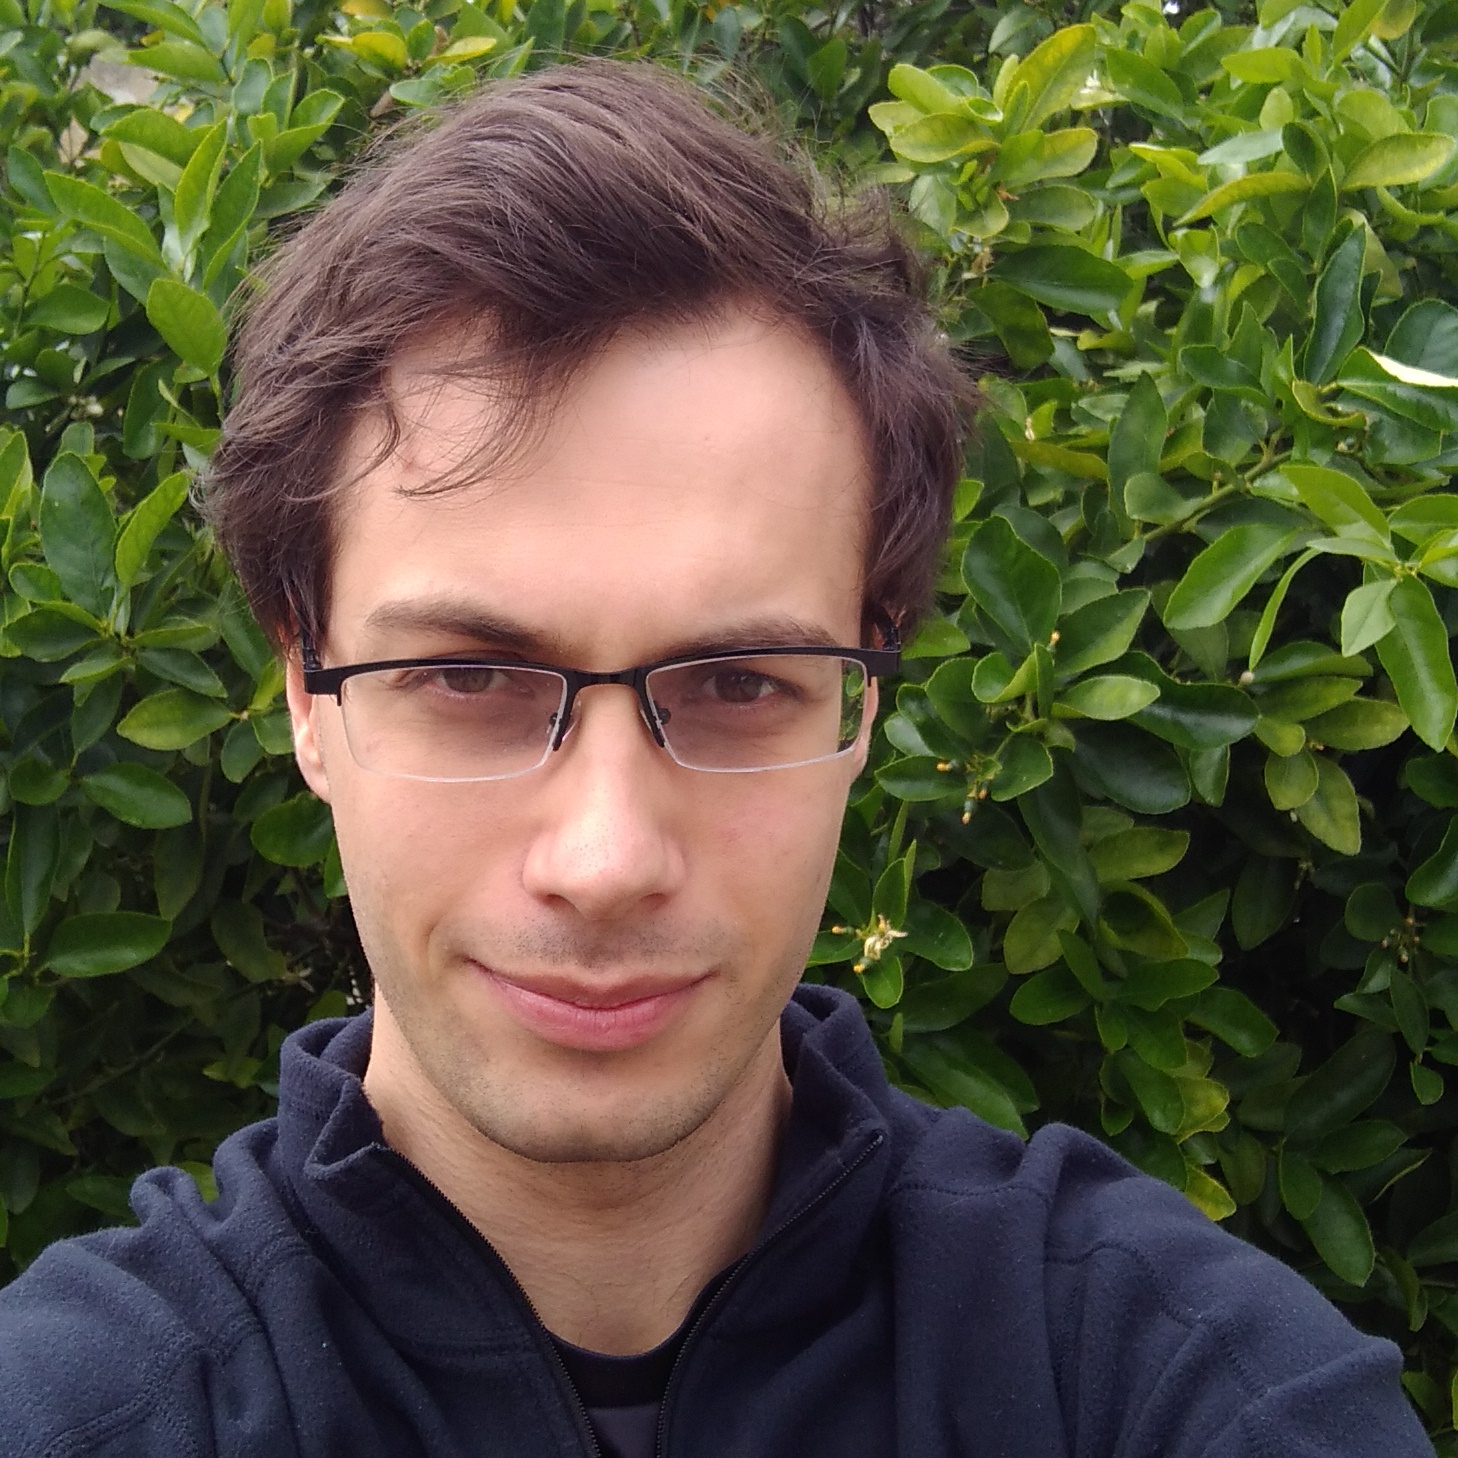
\includegraphics[width=0.5\textwidth]{img/Matthew.jpg}
\vspace{1em}
      \begin{alertblock}{\centering \footnotesize{Matthew Daggitt}}
     \end{alertblock}

          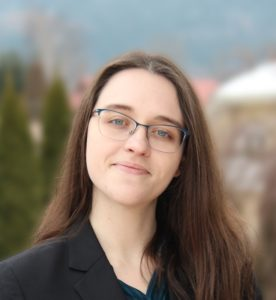
\includegraphics[width=0.5\textwidth]{img/Natalia.jpg}
           \begin{block}{\centering\footnotesize{Natalia Slusarz}}
           \end{block}

 \column{.2\textwidth}
       \centering
\vspace{-5em}
         
\includegraphics[width=0.5\textwidth]{img/Ben.jpg}
           \vspace{4em}
   \begin{block}{\centering\footnotesize{Ben Coke}}
       \end{block}

    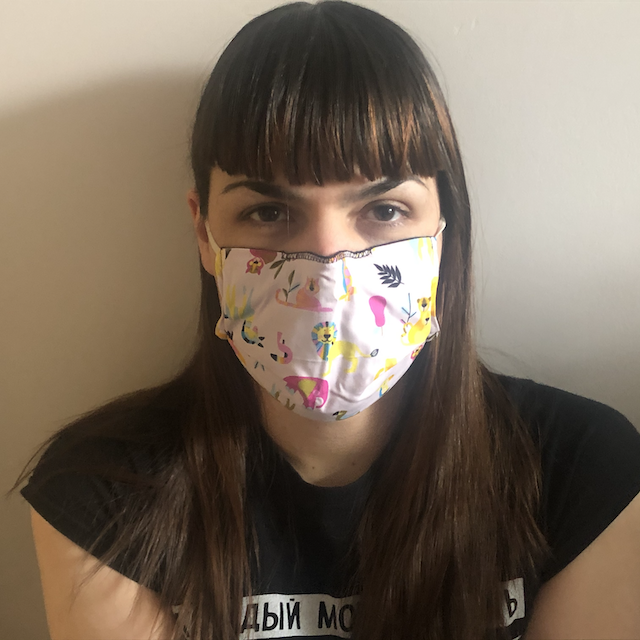
\includegraphics[width=0.5\textwidth]{img/Wen.png}
      \begin{alertblock}{\centering \footnotesize{Wen Kokke}}
   \end{alertblock}

      \column{.2\textwidth}
   \centering
\vspace{-3em}
    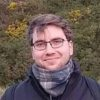
\includegraphics[width=0.5\textwidth]{img/Luca.jpeg}
      \vspace{2em}
    \begin{block}{\centering\footnotesize{Luca Arnaboldi}}
   \end{block}
  
\includegraphics[width=0.5\textwidth]{img/Marco.jpg}
    \vspace{-1em}
        \begin{block}{\centering\footnotesize{Marco Casadio}}
     \end{block}

  %    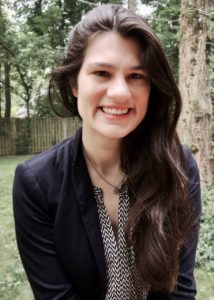
\includegraphics[width=1.5cm]{img/Kathrin.jpg}
  %\begin{block}{\centering\footnotesize{Kathrin Stark}}
  % \end{block}

 \column{.2\textwidth}
  \vspace{-2em}
   \centering
     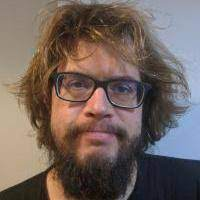
\includegraphics[width=0.5\textwidth]{img/Bob.jpeg}
%\vspace{2em}
         % \includegraphics[width=2cm]{photoDP.jpg}
           \vspace{1em}
          \begin{block}{\centering\footnotesize{Bob Atkey}}
     \end{block}

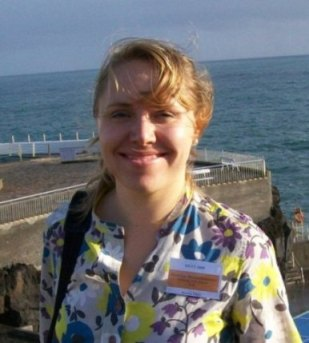
\includegraphics[width=0.5\textwidth]{img/Katya3.jpg}
\vspace{-1em}
\begin{block}{\centering\footnotesize{Katya K}}
   \end{block}

\column{.2\textwidth}
   \centering
   %\vspace{-2em}
  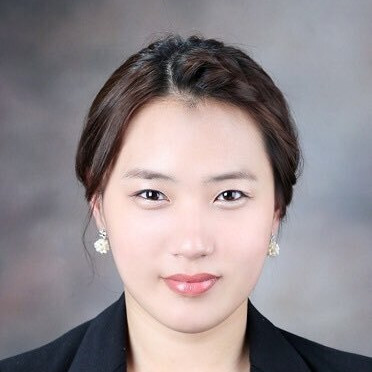
\includegraphics[width=0.5\textwidth]{img/JL.jpeg}
\begin{block}{\centering\footnotesize{Jeonghyeon Lee}}
   \end{block}
  \end{columns}
%  \end{center}
  \end{frame}




\section{Neural Network Verification: overview of the new domain}


\begin{frame}
\frametitle{Neural nets for classification}
\centering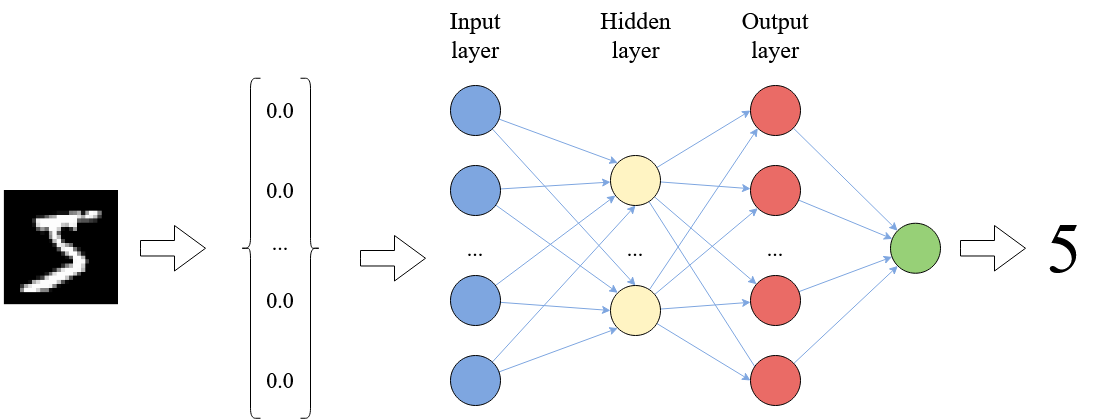
\includegraphics[scale=.30]{img/mnist_classification.png}

\begin{block}{Formally,}
 a neural network is a function $N : R^n \rightarrow R^m$.
\end{block}

\end{frame}

\begin{frame}
\frametitle{Neural networks}

\begin{alertblock}{... are ideal for  ``perception'' tasks:}
    \setbeamercovered{transparent}
\begin{itemize}[<+->]
  \item approximate functions when exact solution is hard to get
    \item tolerant to noisy and incomplete data
    \end{itemize}
\end{alertblock}
\pause

\begin{block}{BUT}
  \begin{itemize}
   % \item continuous decision space means solutions can only be approximate
	\item solutions not easily conceptualised (\alert{lack of explainability})
	%\item prone to error
	\item prone to a new range of safety and security problems: \pause
          \begin{itemize} \item[] adversarial attacks
        \item[]  data poisoning
        \item[] catastrophic forgetting
          \end{itemize}
\end{itemize}
\end{block}
\end{frame}

\begin{frame}
  \frametitle{One example: Adversarial Attacks}

 % \begin{block}{}
 %   Given a trained neural network and a correctly classified image of ``0'' on the left,
 %                 we can create a perturbation $\eta$ (middle) to the original image so that the same neural network predicts a ``5" with 92\% confidence for the modified image (right).
 %   \end{block}

  	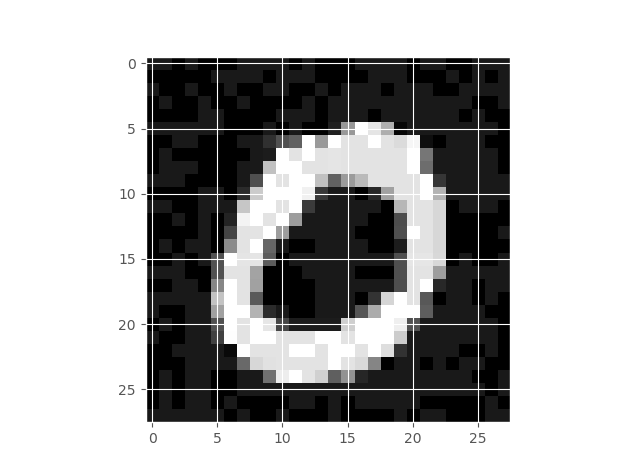
\includegraphics[width=.3\textwidth]{img/true.png}
	\uncover<2->{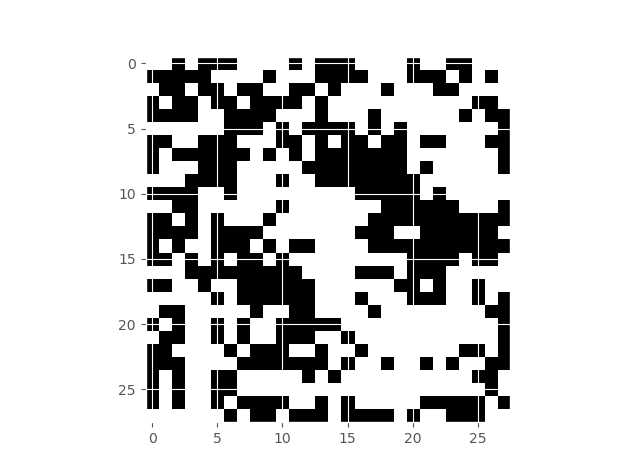
\includegraphics[width=.3\textwidth]{img/eta.png}}
	\uncover<3->{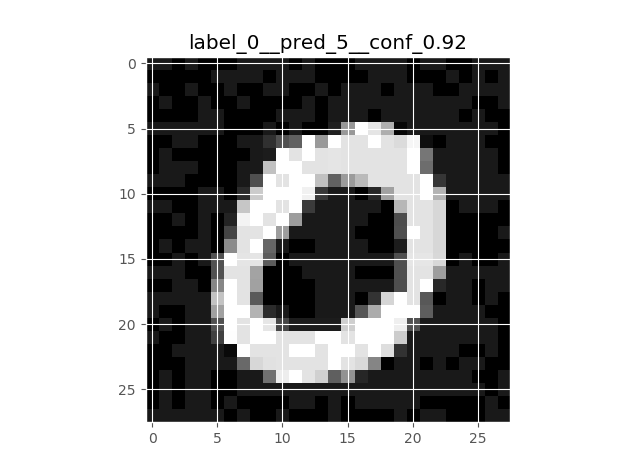
\includegraphics[width=.3\textwidth]{img/adv.png}}

\begin{itemize}
\item<4->[] the perturbations are imperceptible to human eye \pause
\item<5->[] attacks transfer from one neural network to another \pause
\item<6->[] affect any domain where neural networks are applied
\end{itemize}

\end{frame}

\begin{frame}
      \frametitle{Verification Property:  ``$\epsilon$-ball robustness''}

    \vspace{-2em}
\begin{center}
  \begin{tikzpicture}[scale=.65]
  % draw the sphere
  \shade[ball color = gray!40, opacity = 0.4] circle (2cm);
  \draw (0,0) circle (2cm);
  \draw (-2,0) arc (180:360:2 and 1);
  \draw[dashed] (2,0) arc (0:180:2 and 1);
  \fill[fill=black] (0,0) circle (1pt);
  \draw[dashed,<->] (0,0 ) -- node[above]{$\epsilon$} (2,0);
  % line for original image
  \draw[] (0,0 ) -- node{} (0,-2.5);
  \node (1orig) at (0,-3) {
\includegraphics{img/7_orig.png}};
 % \node[] at (0,-3.8) {NN: ``seven''};
  % line for the perturbed image 1
  \draw[] (-0.6,1.2) -- node{} (-0.9,2.7);
  \node () at (-1,2.8) {
\includegraphics{img/7_v1}};
  % line for the perturbed image 2
  \draw[] (0.6,1.4) -- node{} (1.2,2.7);
  \node () at (1.2,2.8) {
\includegraphics{img/7_v2}};
  % line for the perturbed image 3
  \draw[] (0.6,-1.2) -- node{} (2.5,-2.7);
  \node () at (2.5,-2.8) {
\includegraphics{img/7_v3}};
\end{tikzpicture}
\end{center}


  \small{\begin{alertblock}{An $\epsilon$-ball     $\mathbb{B}(\hat{\mathbf{x}}, \epsilon) = \{ {\mathbf{x} \in \mathbb{R}^n: |\hat{\mathbf{x}}-\mathbf{x}| \leq \epsilon} \}$ }


    Classify all  points in $\mathbb{B}(\hat{\mathbf{x}}, \epsilon)$ ``robustly''.
    %in the \alert{``same class''} as $\hat{\mathbf{x}}$.
  \end{alertblock}}

 % \begin{block}{}
%\end{block}
    \end{frame}


    \begin{frame}
\frametitle{Another example property: ACAS Xu}
A collision avoidance system for unmanned autonomous aircraft.
\tikz [remember picture,overlay]{
\node at ([xshift=3cm,yshift=3cm]current page.south) {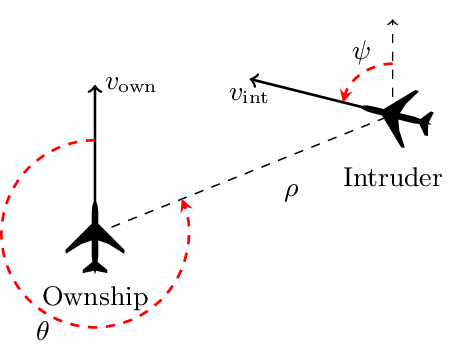
\includegraphics[width=0.5\linewidth]{img/acas_xu.png}};}

{\small
Inputs:
\vspace{-0.7em}
\begin{itemize}
\setlength\itemsep{-0.1em}
\item Distance to intruder, $\rho$
\item Angle to intruder, $\theta$
\item Intruder heading, $\varphi$
\item Speed, $v_{own}$
\item Intruder speed, $v_{int}$
\end{itemize}


Outputs:
\vspace{-0.7em}
\begin{itemize}
\setlength\itemsep{-0.1em}
\item Clear of conflict
\item Strong left
\item Weak left
\item Weak right
\item Strong right
\end{itemize}}

\end{frame}


\begin{frame}
\frametitle{ACAS Xu}
The system was originally implemented as a 2Gb lookup table but was replaced with a neural network in order to improve size and latency requirements.

\pause
\alert{10 different specified properties in total.}

\pause
\begin{definition}[ACAS Xu: Property 1]
\emph{If the intruder is distant and is significantly slower than the ownship, the score of a COC advisory will always be below a certain fixed threshold.}
\end{definition}

\pause
\begin{block}{}
\begin{equation*}
\begin{array}{l}
(\rho \geq 55947.691) \wedge
(v_{own} \geq 1145) \wedge (v_{int} \leq 60)  \\
\Rightarrow \text{the score for COC is at most 1500}
\end{array}
\end{equation*}
\end{block}

\end{frame}

    \begin{frame}
    \frametitle{More Generally}

    \begin{block}{Given $N : R^n \rightarrow R^m$}
    Verification of such functions most commonly boils down to specifying admissible intervals for the function's output given an interval for its inputs.
\end{block}
  \uncover<2->{
    {\footnotesize
 \begin{thebibliography}{99}
 \beamertemplatearticlebibitems
\bibitem{1}{Casadio, M., Komendantskaya, E., Daggitt, M.L., Kokke, W., Katz, G., Amir, G., Refaeli, I.:
Neural network robustness as a verification property: A principled case study. In: Computer
Aided Verification (CAV 2022).}
 \end{thebibliography}}}

    \end{frame}

\begin{frame}{Overview of The Verification Landscape}%{Problem Statement}
% \centering<1>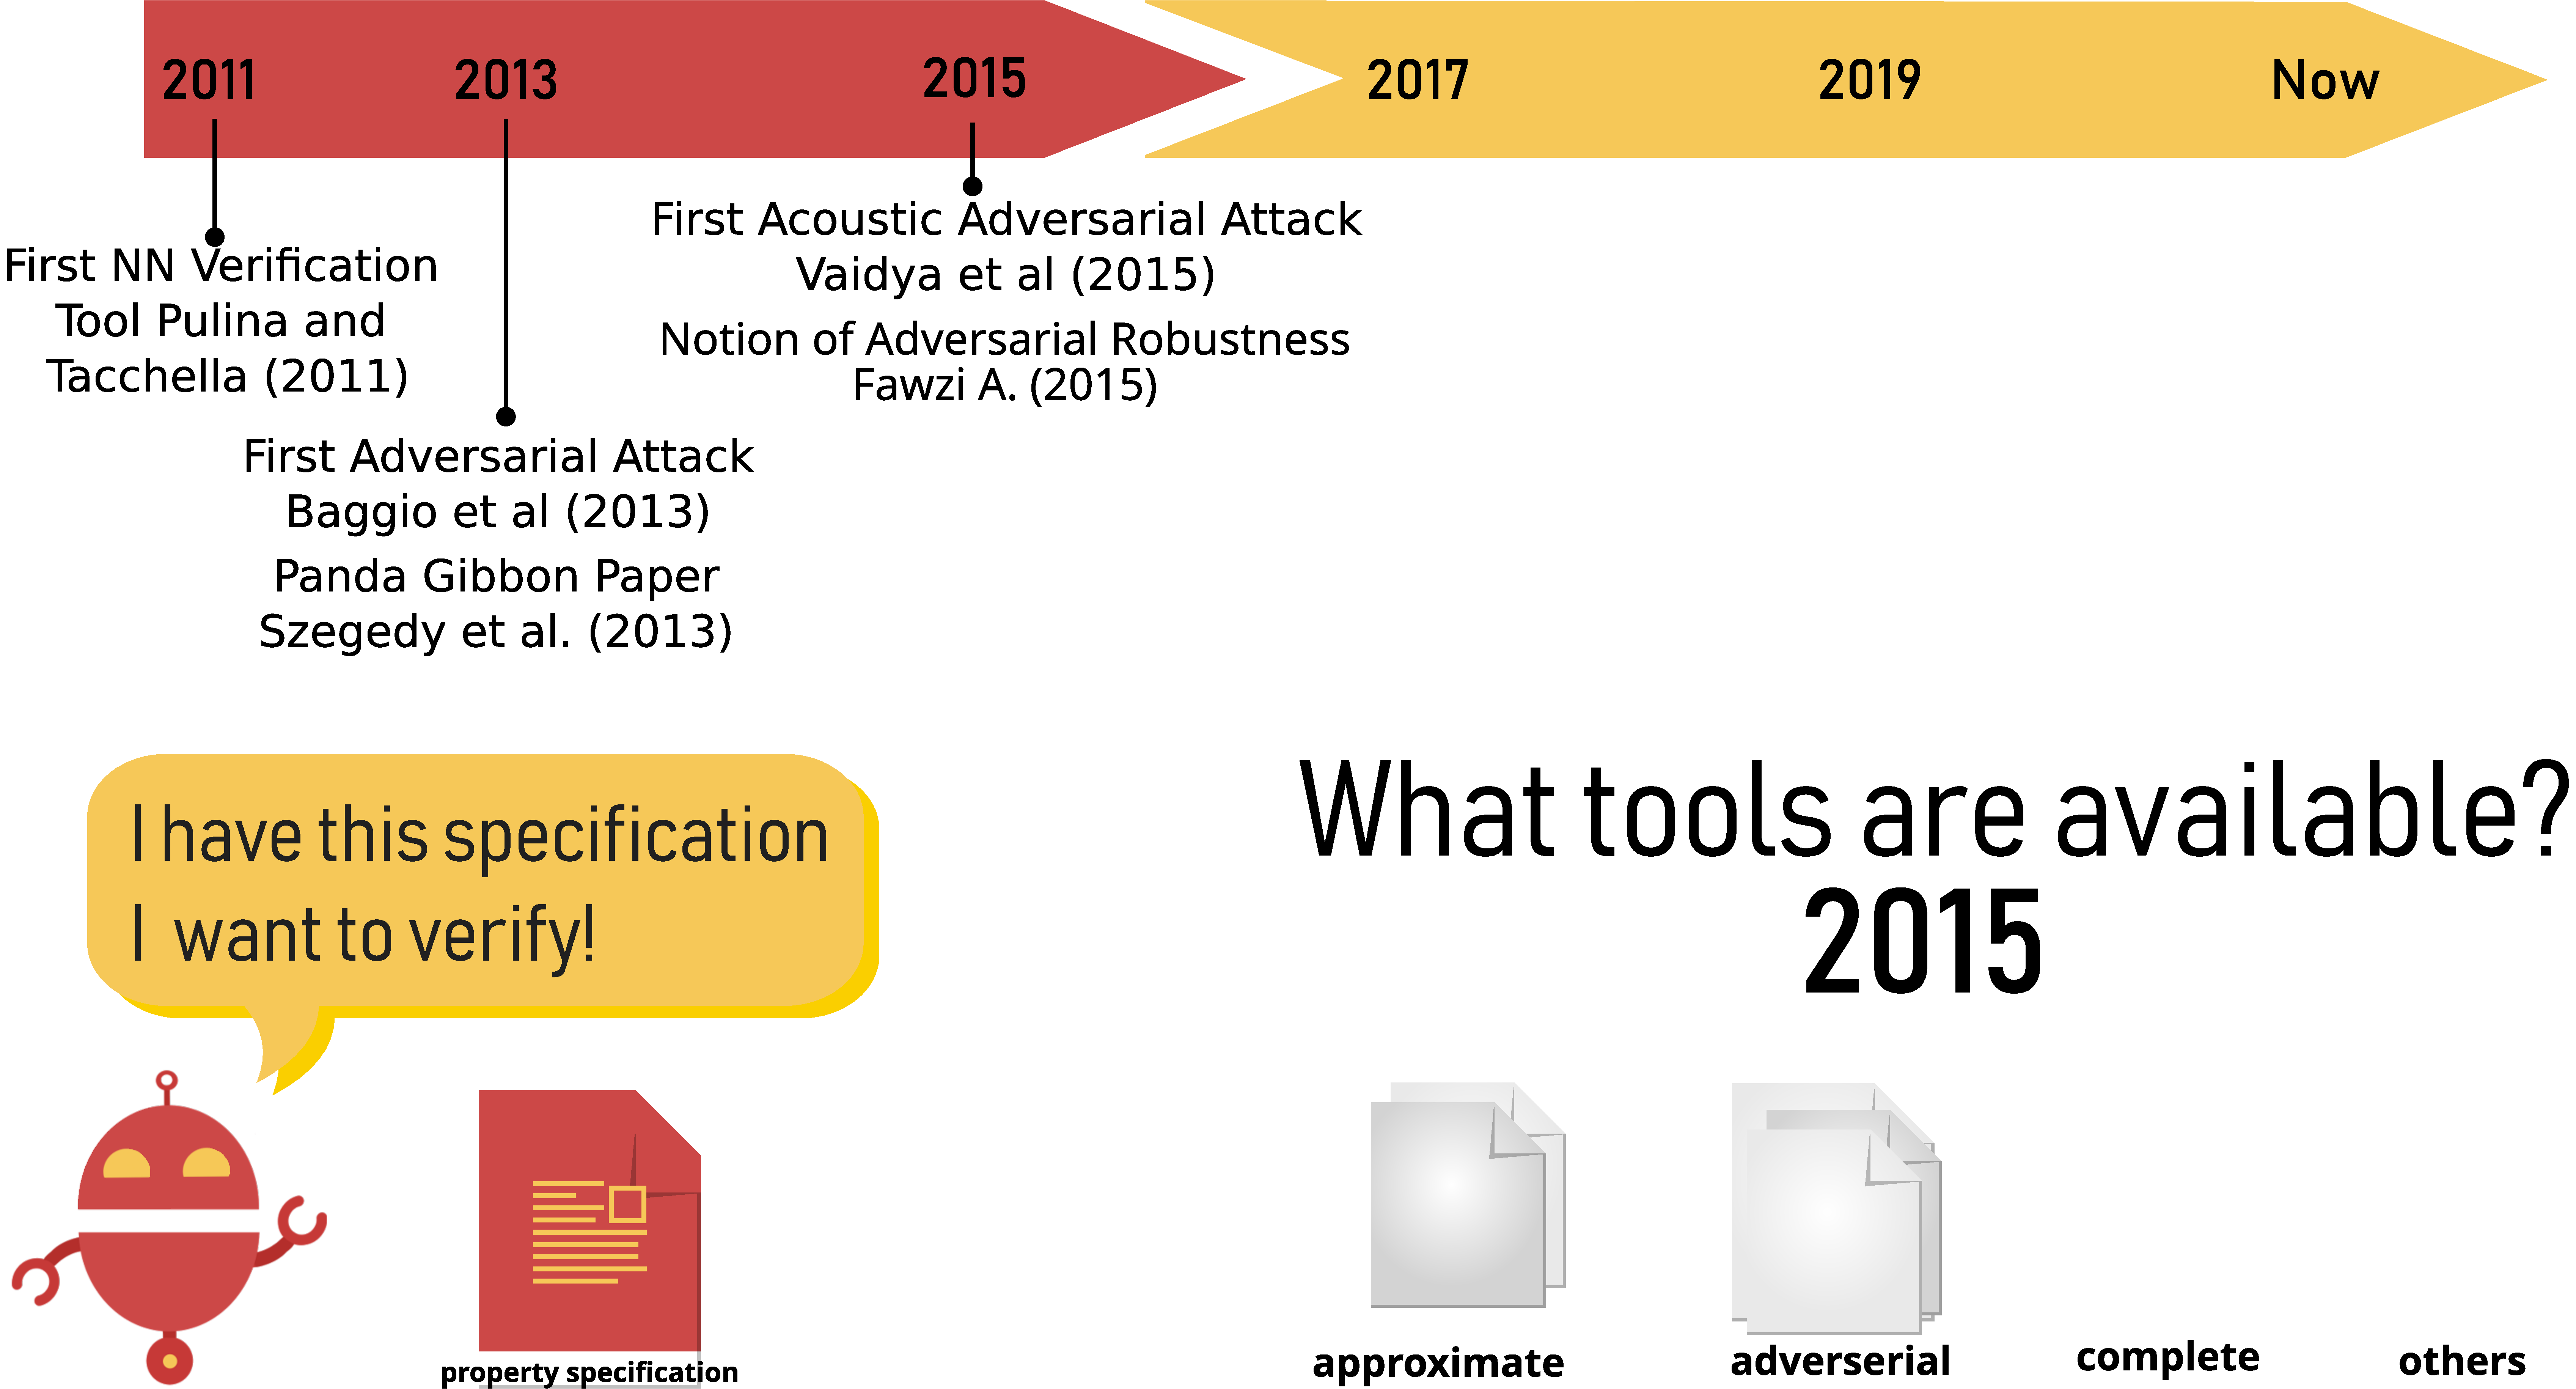
\includegraphics[width=0.8\textwidth]{img/first-slide-2015.pdf}
% \centering<2>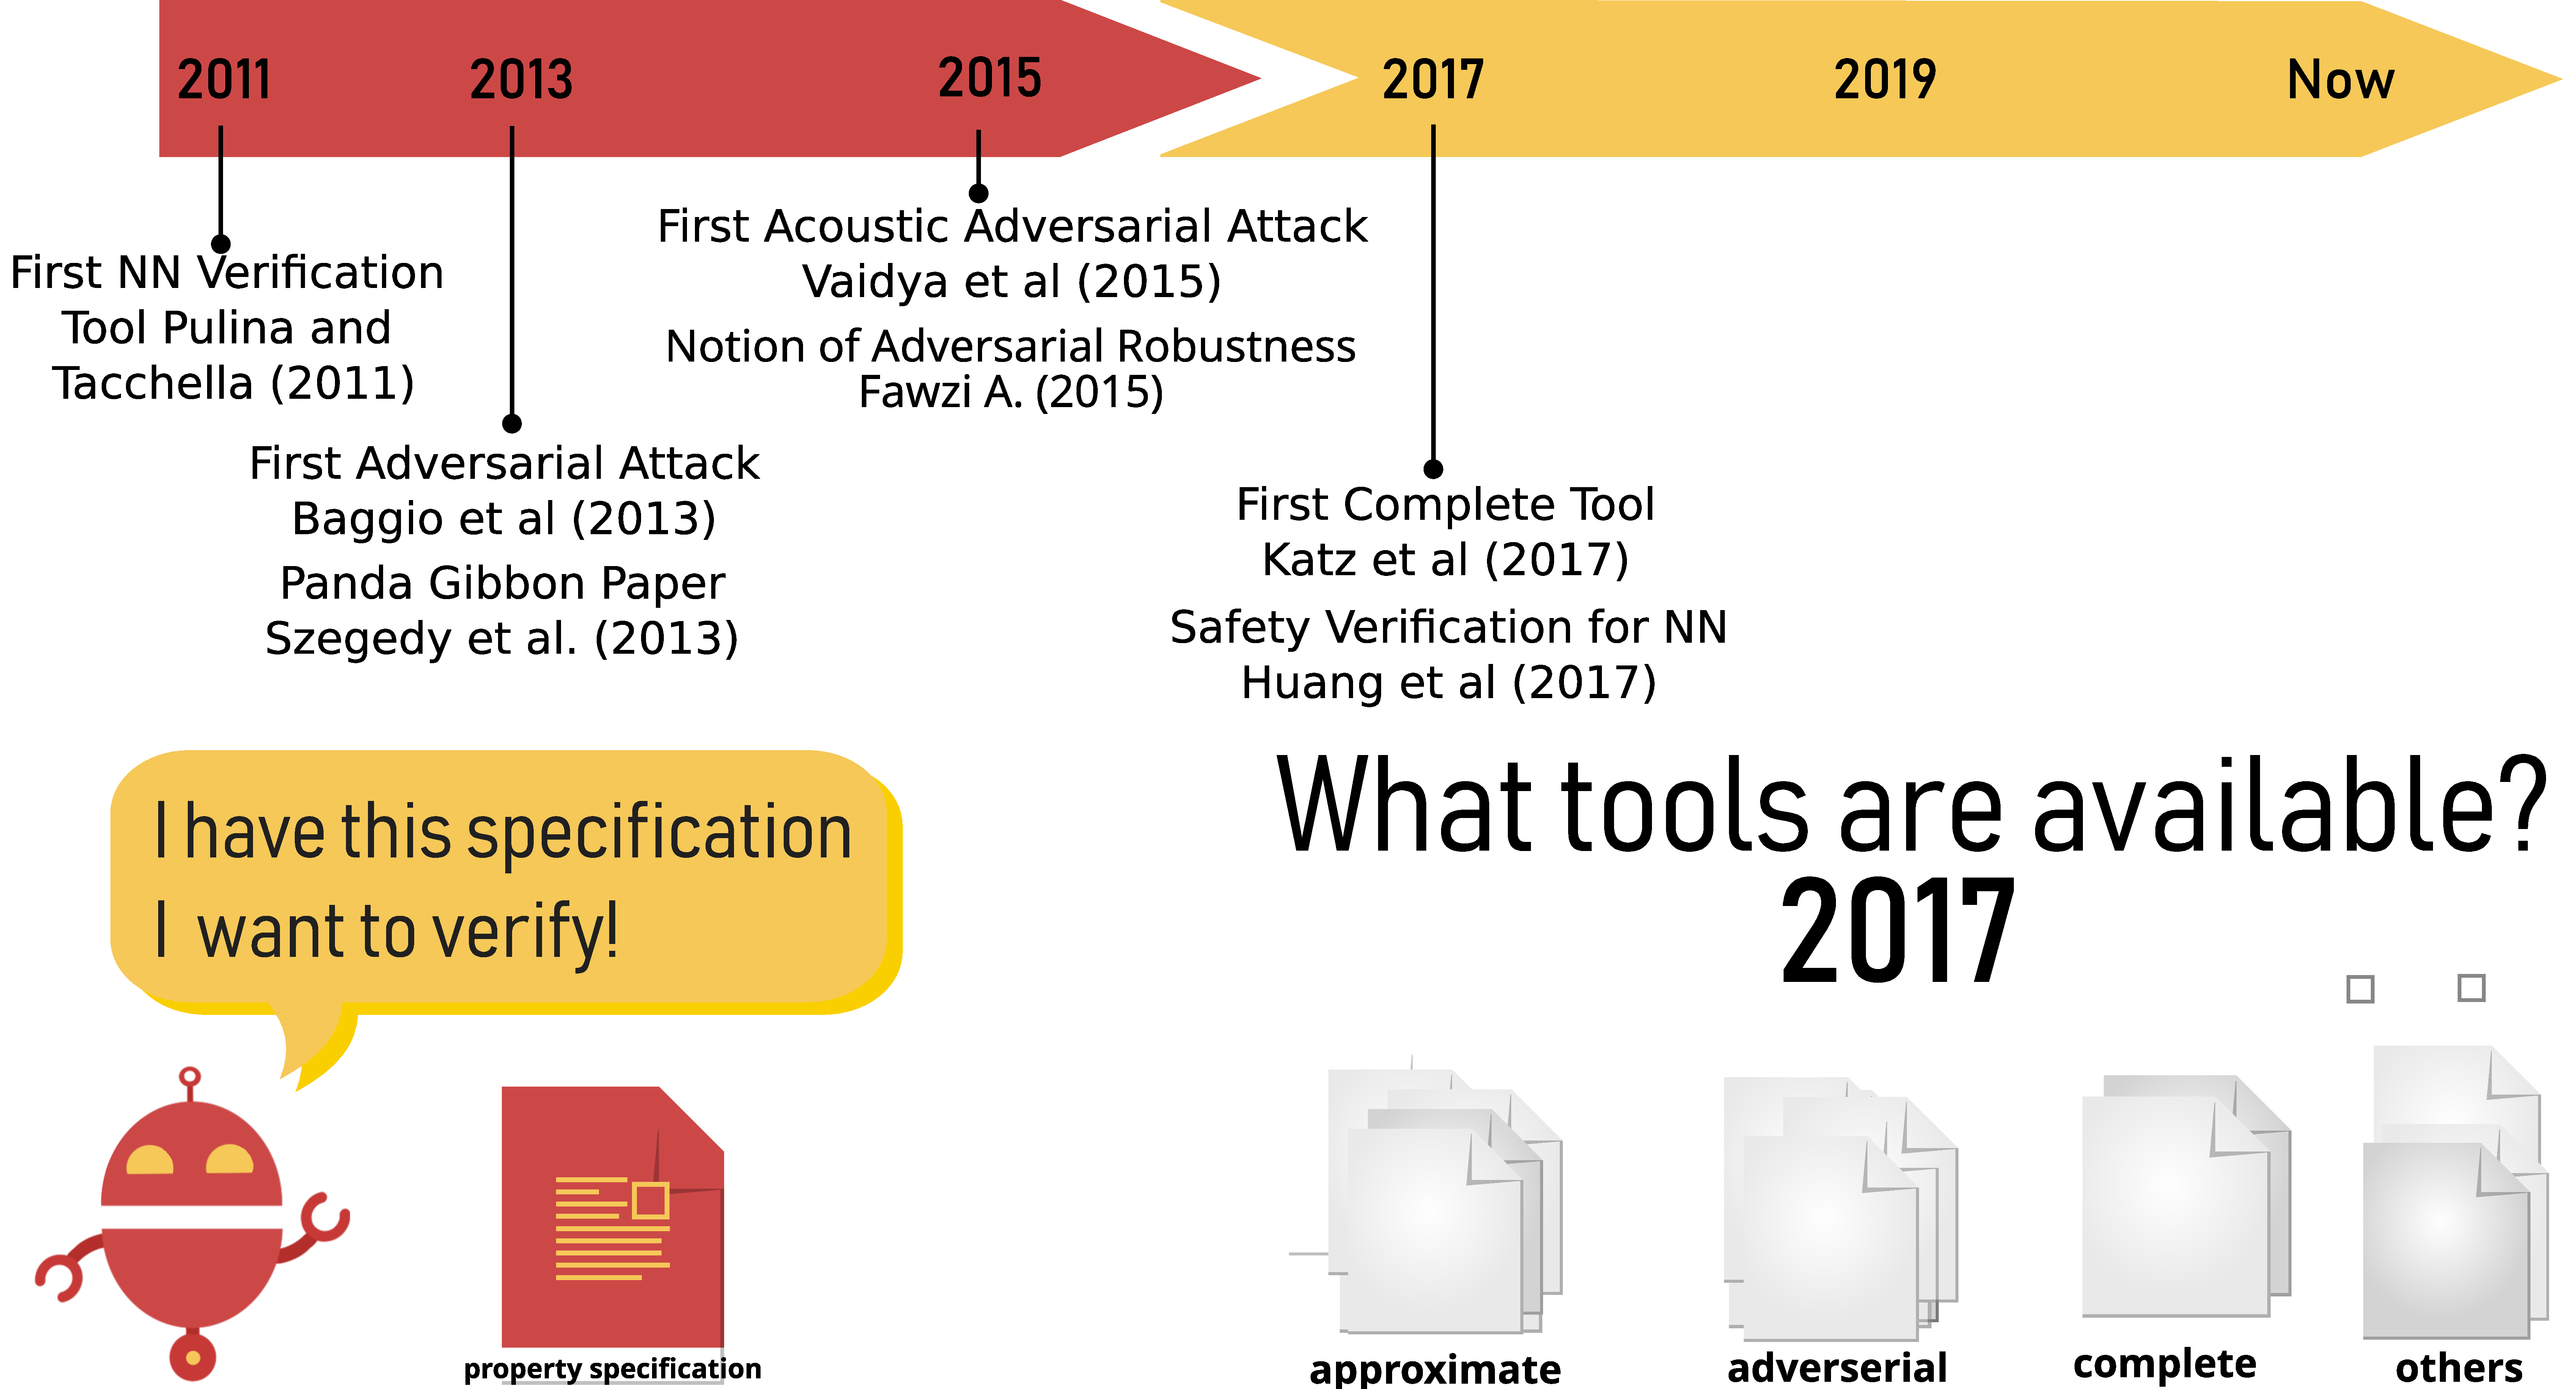
\includegraphics[width=0.8\textwidth]{img/first-slide-2017.pdf}
% \centering<3>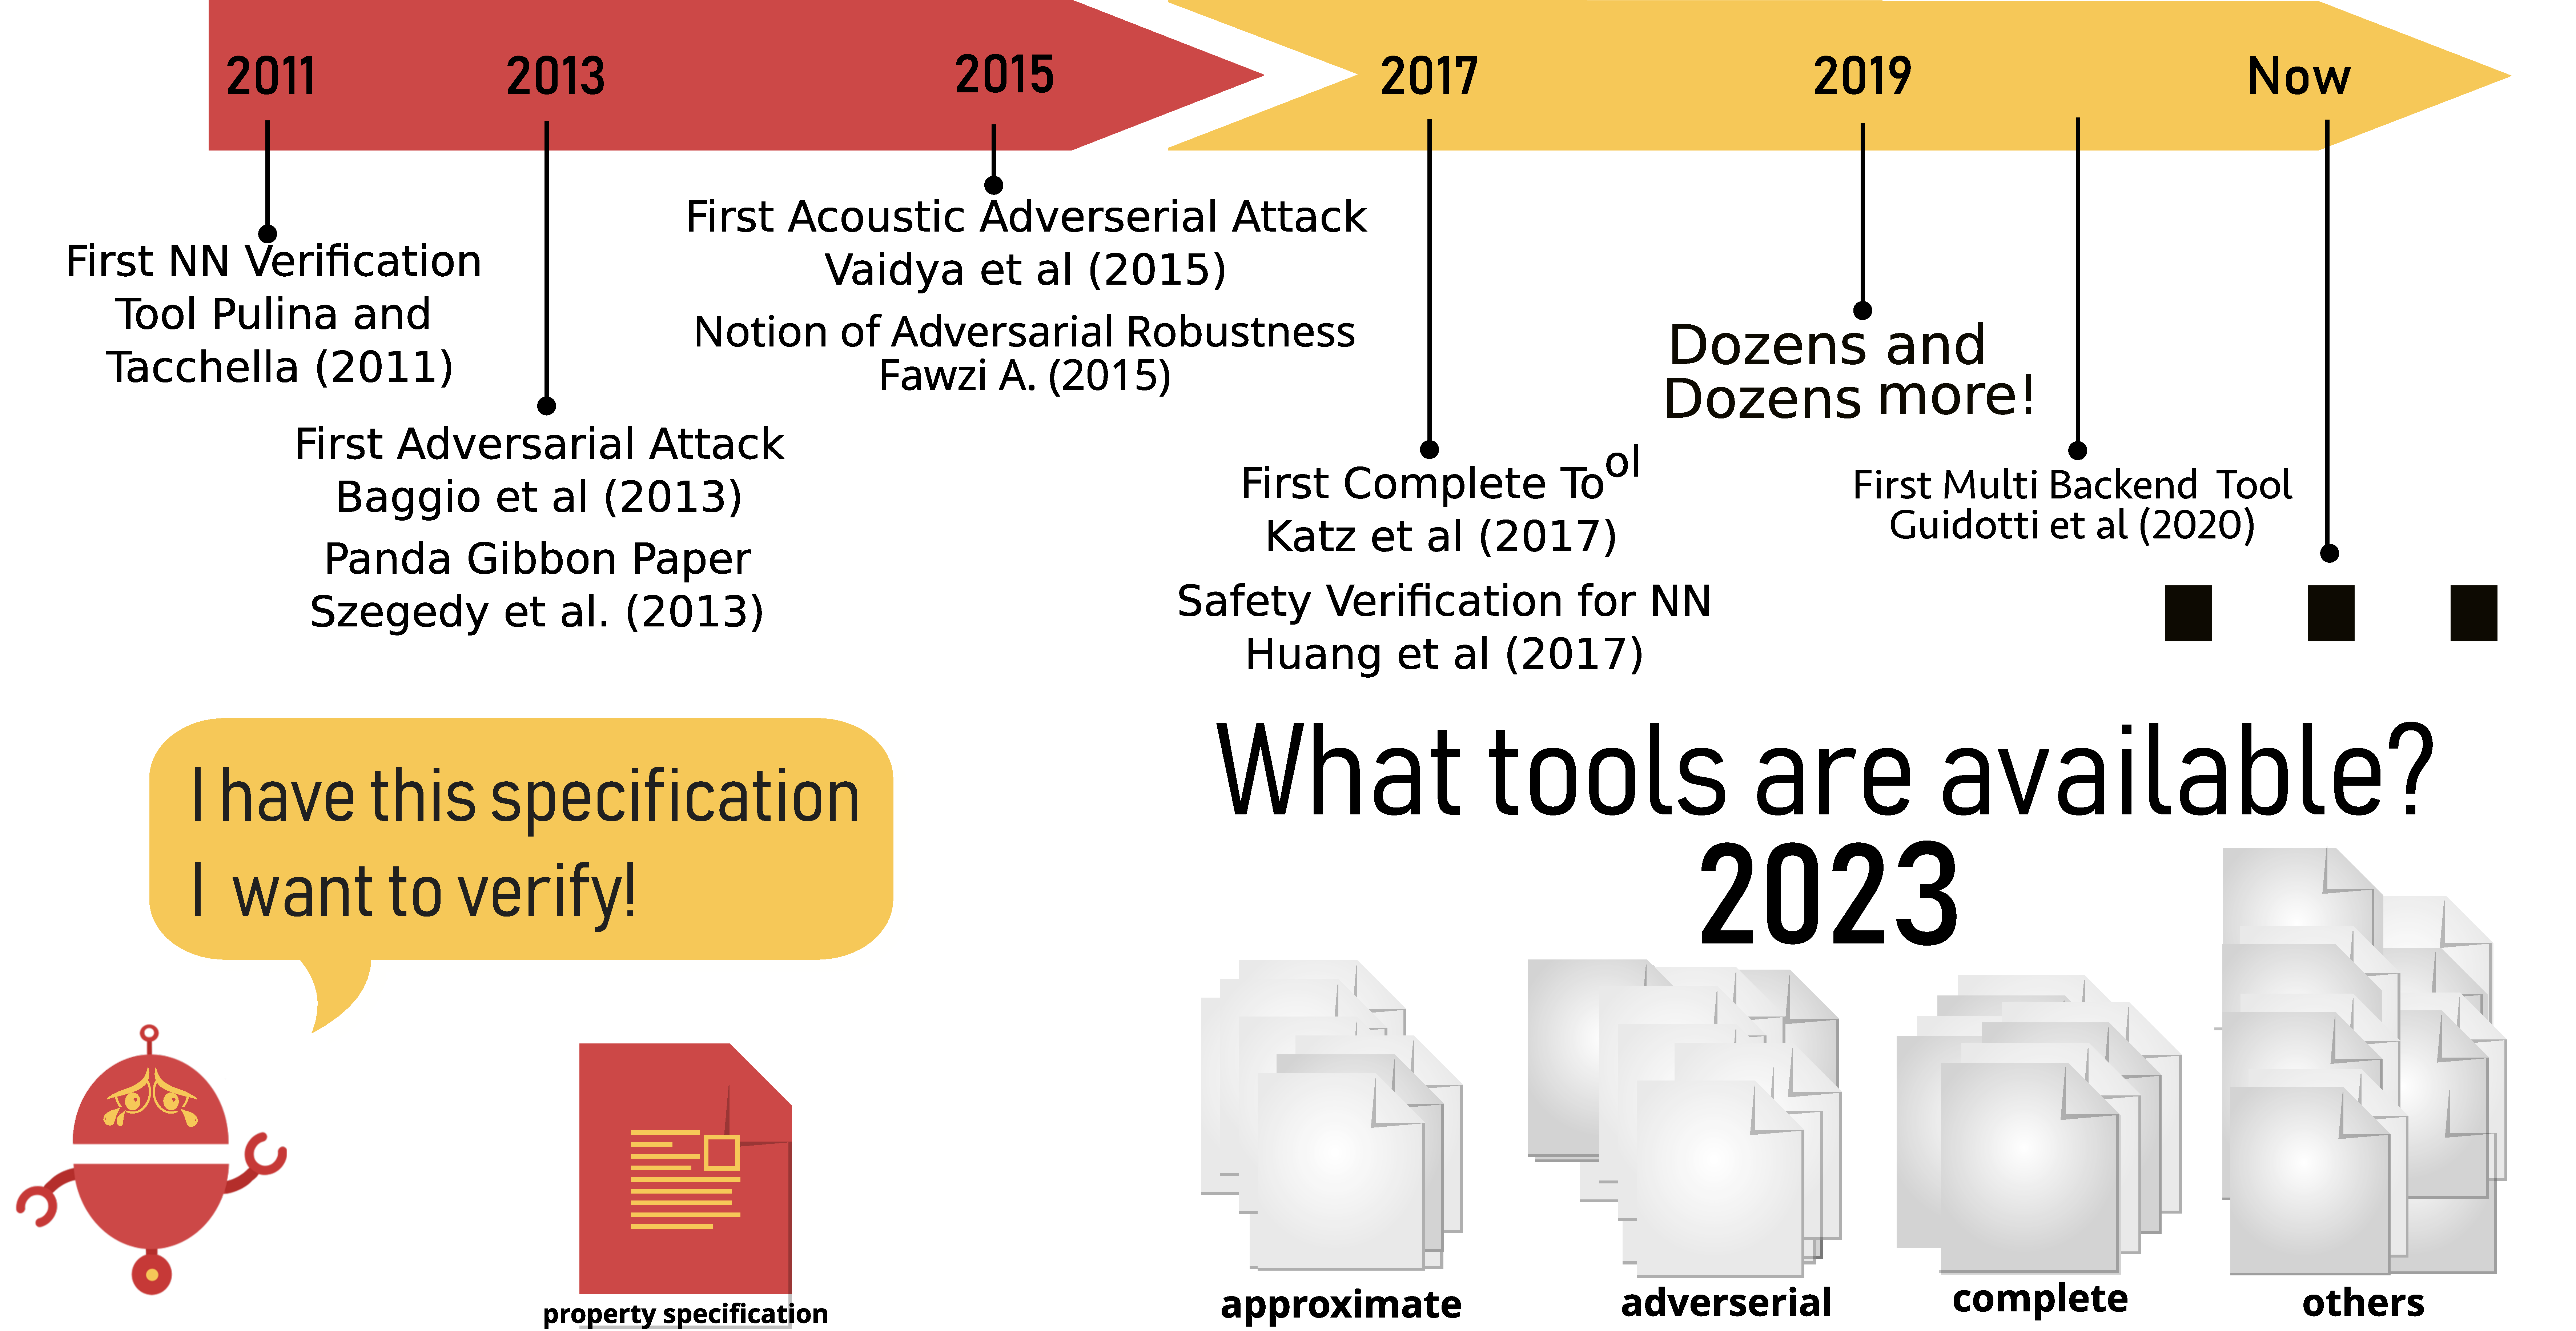
\includegraphics[width=0.8\textwidth]{img/first-slide-2022.pdf}
\only<1>{\vspace{-0.5cm}\centering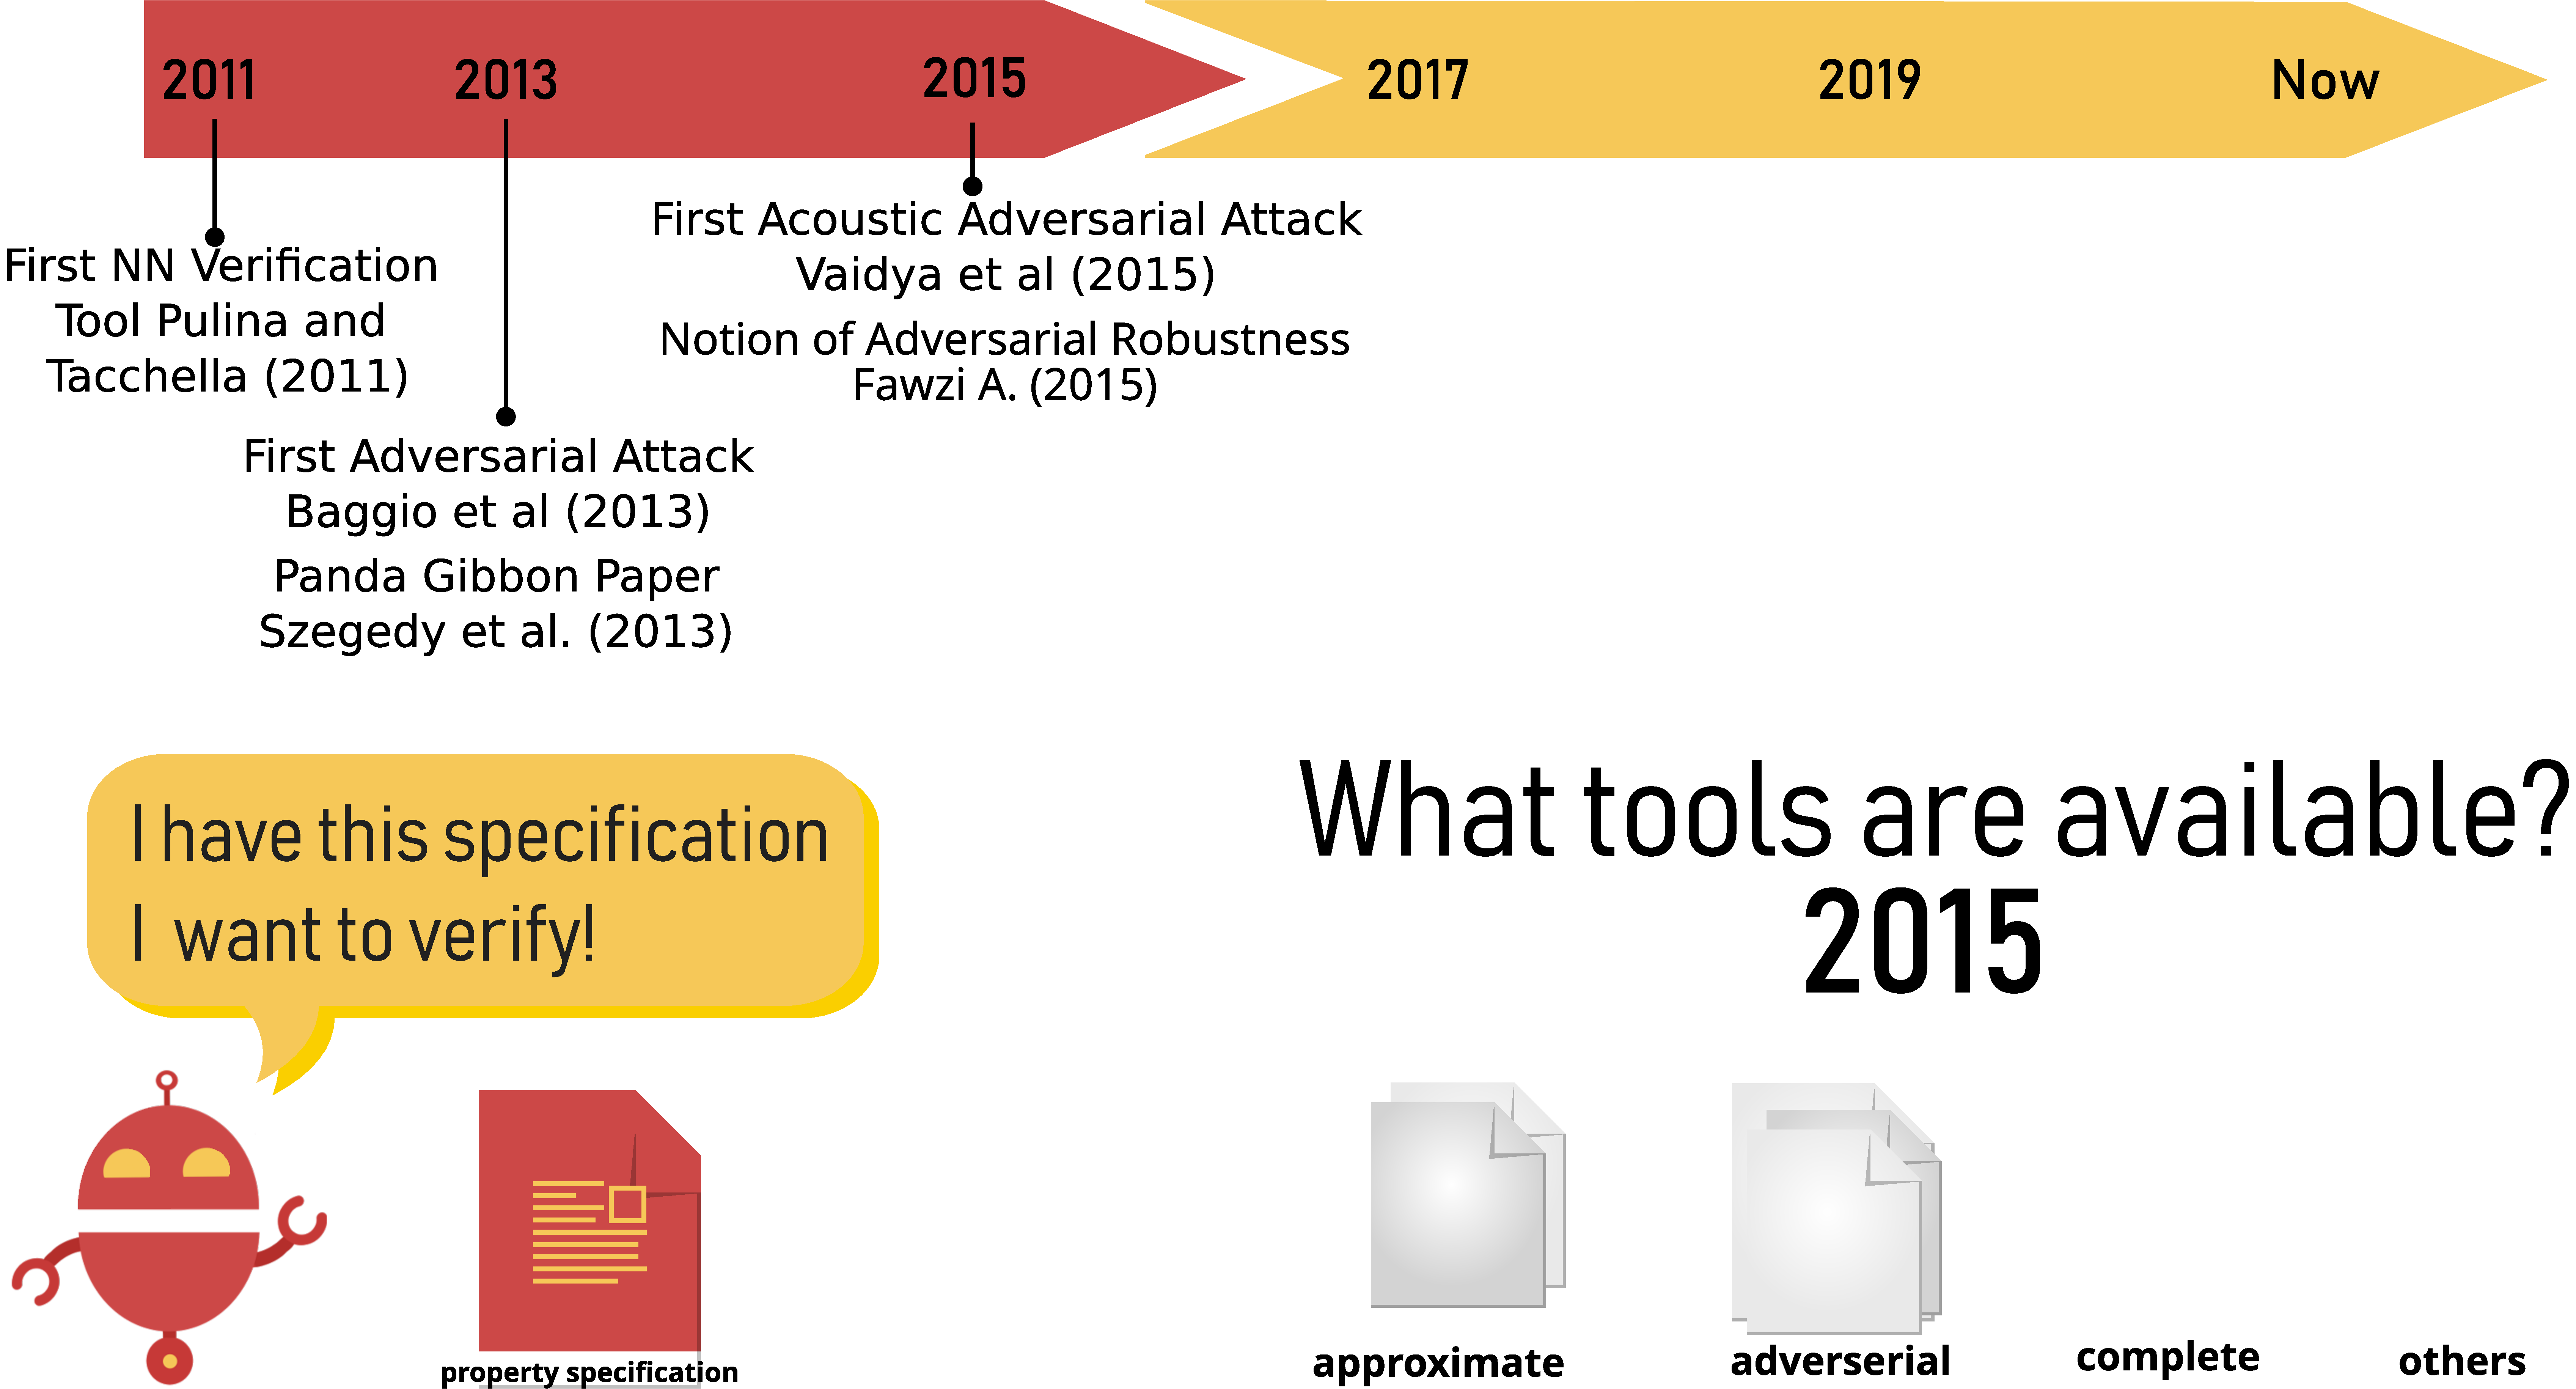
\includegraphics[width=0.9\textwidth]{img/first-slide-2015.pdf}}
\only<2>{\vspace{-0.5cm}\centering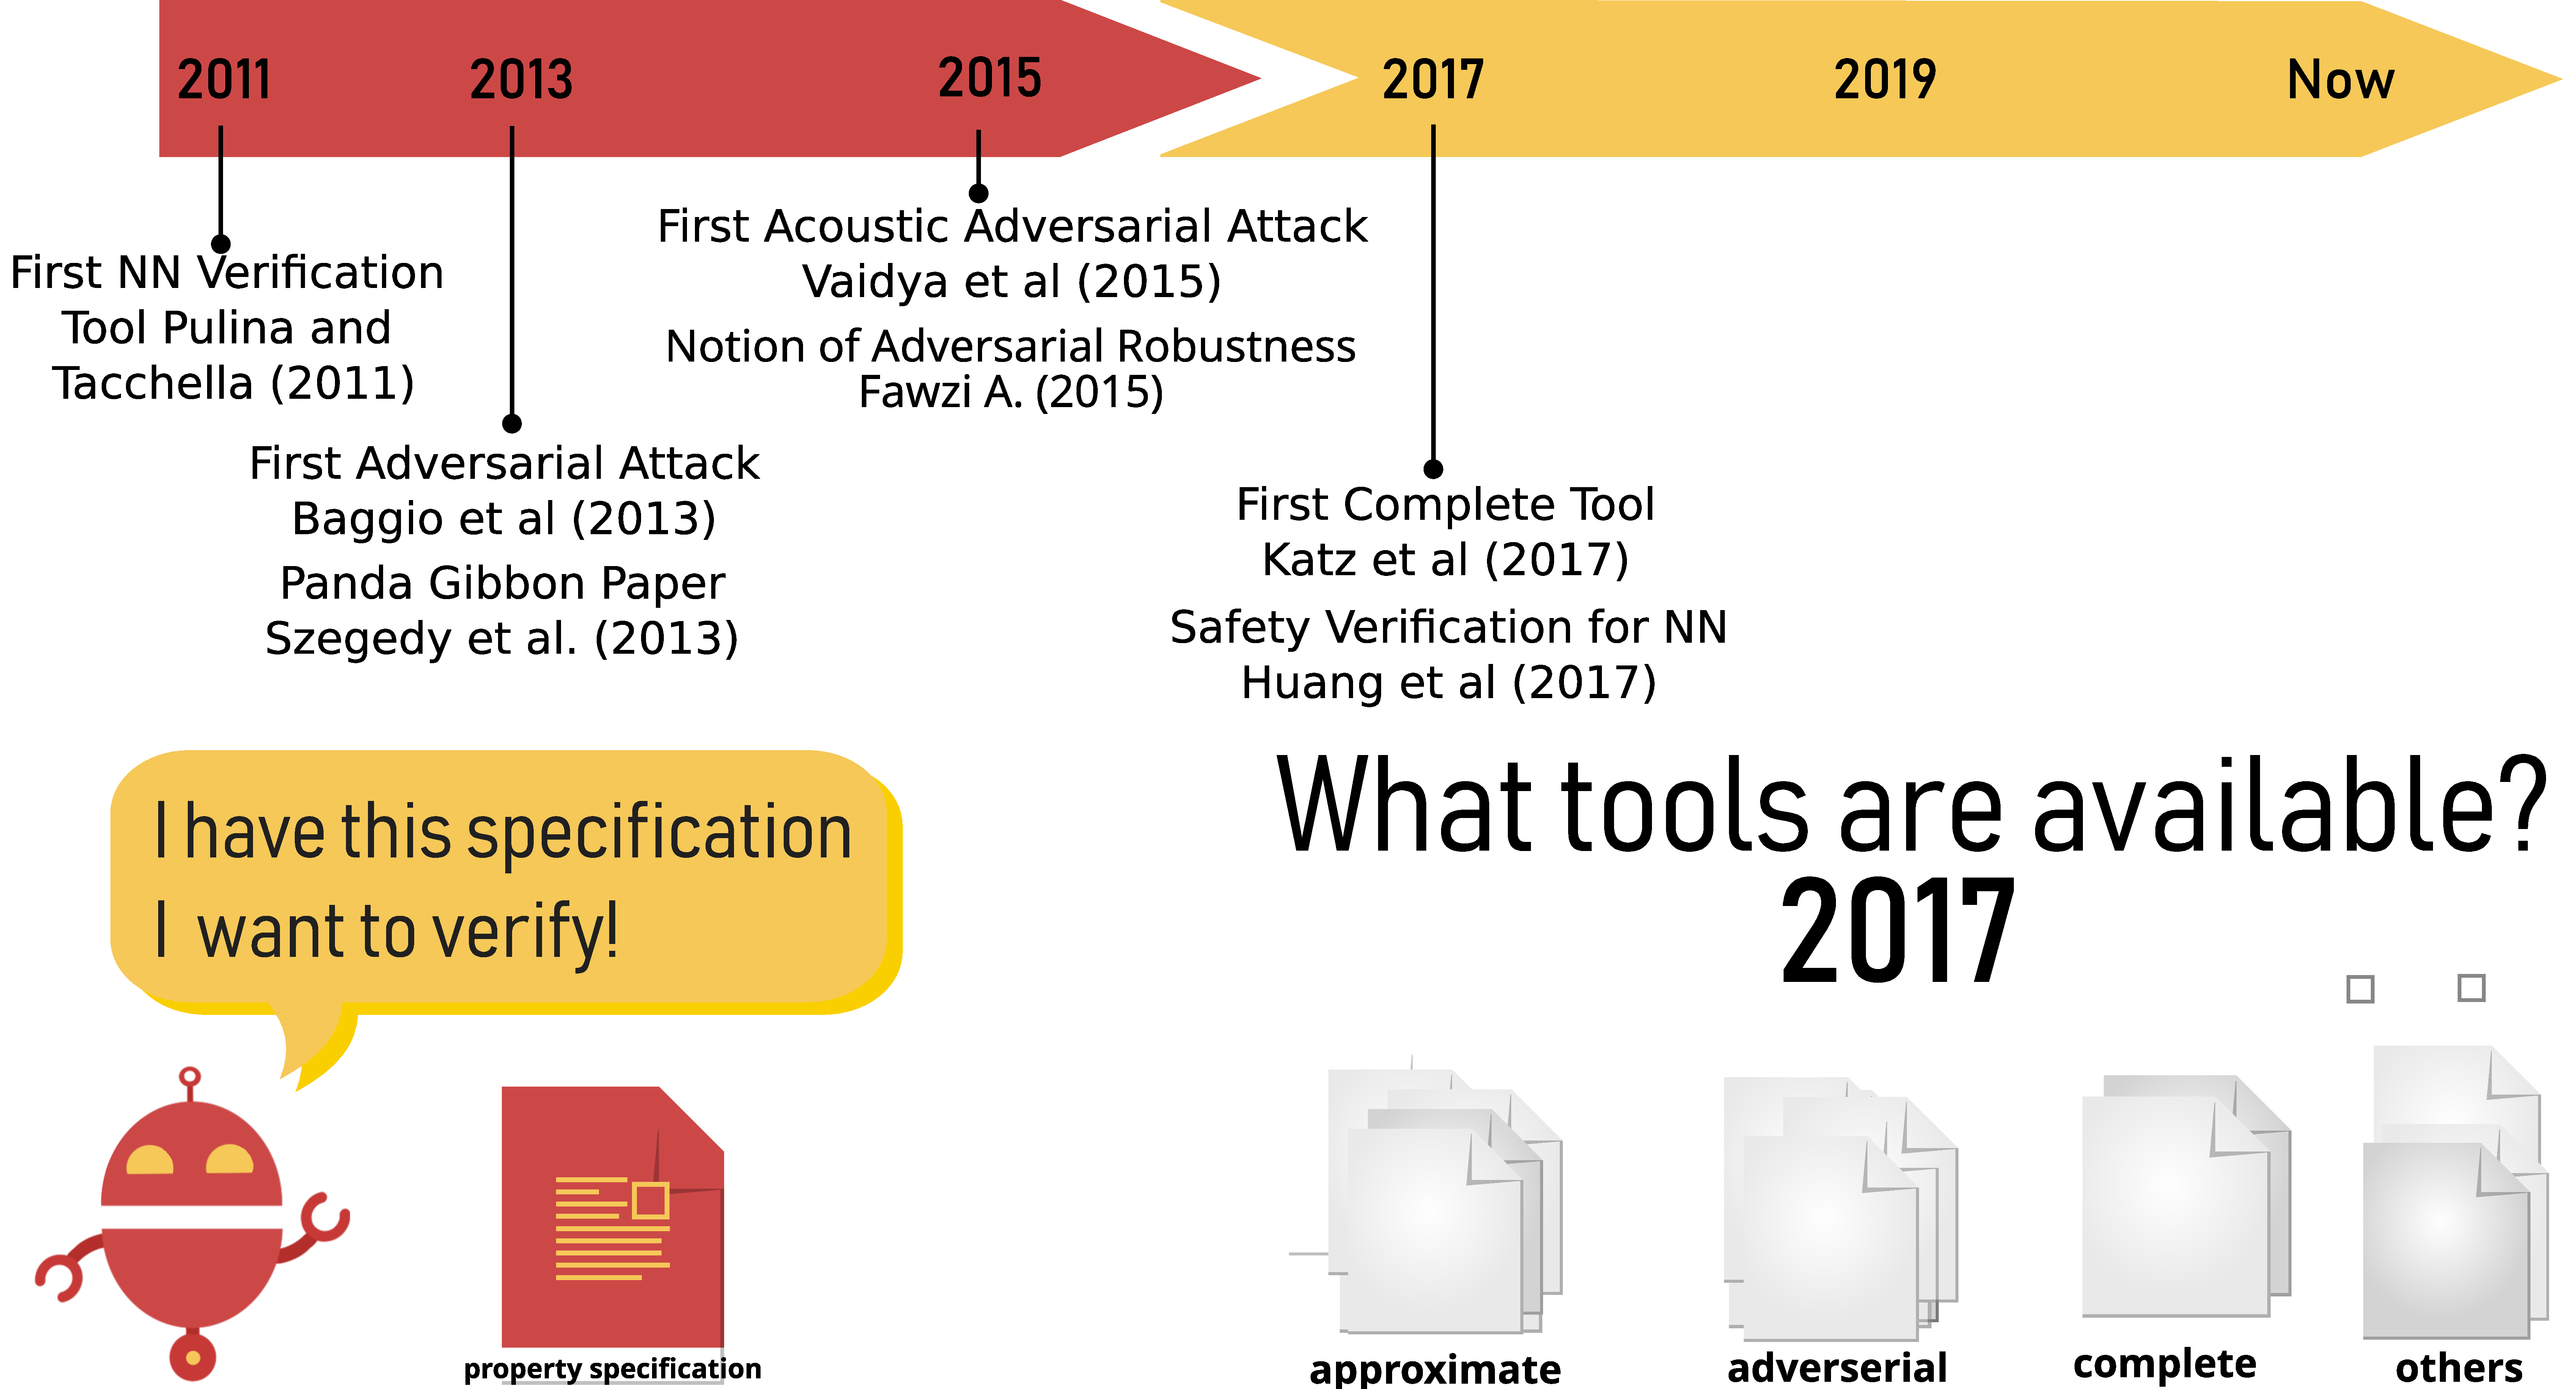
\includegraphics[width=0.9\textwidth]{img/first-slide-2017.pdf}}
\only<3>{\vspace{-0.5cm}\centering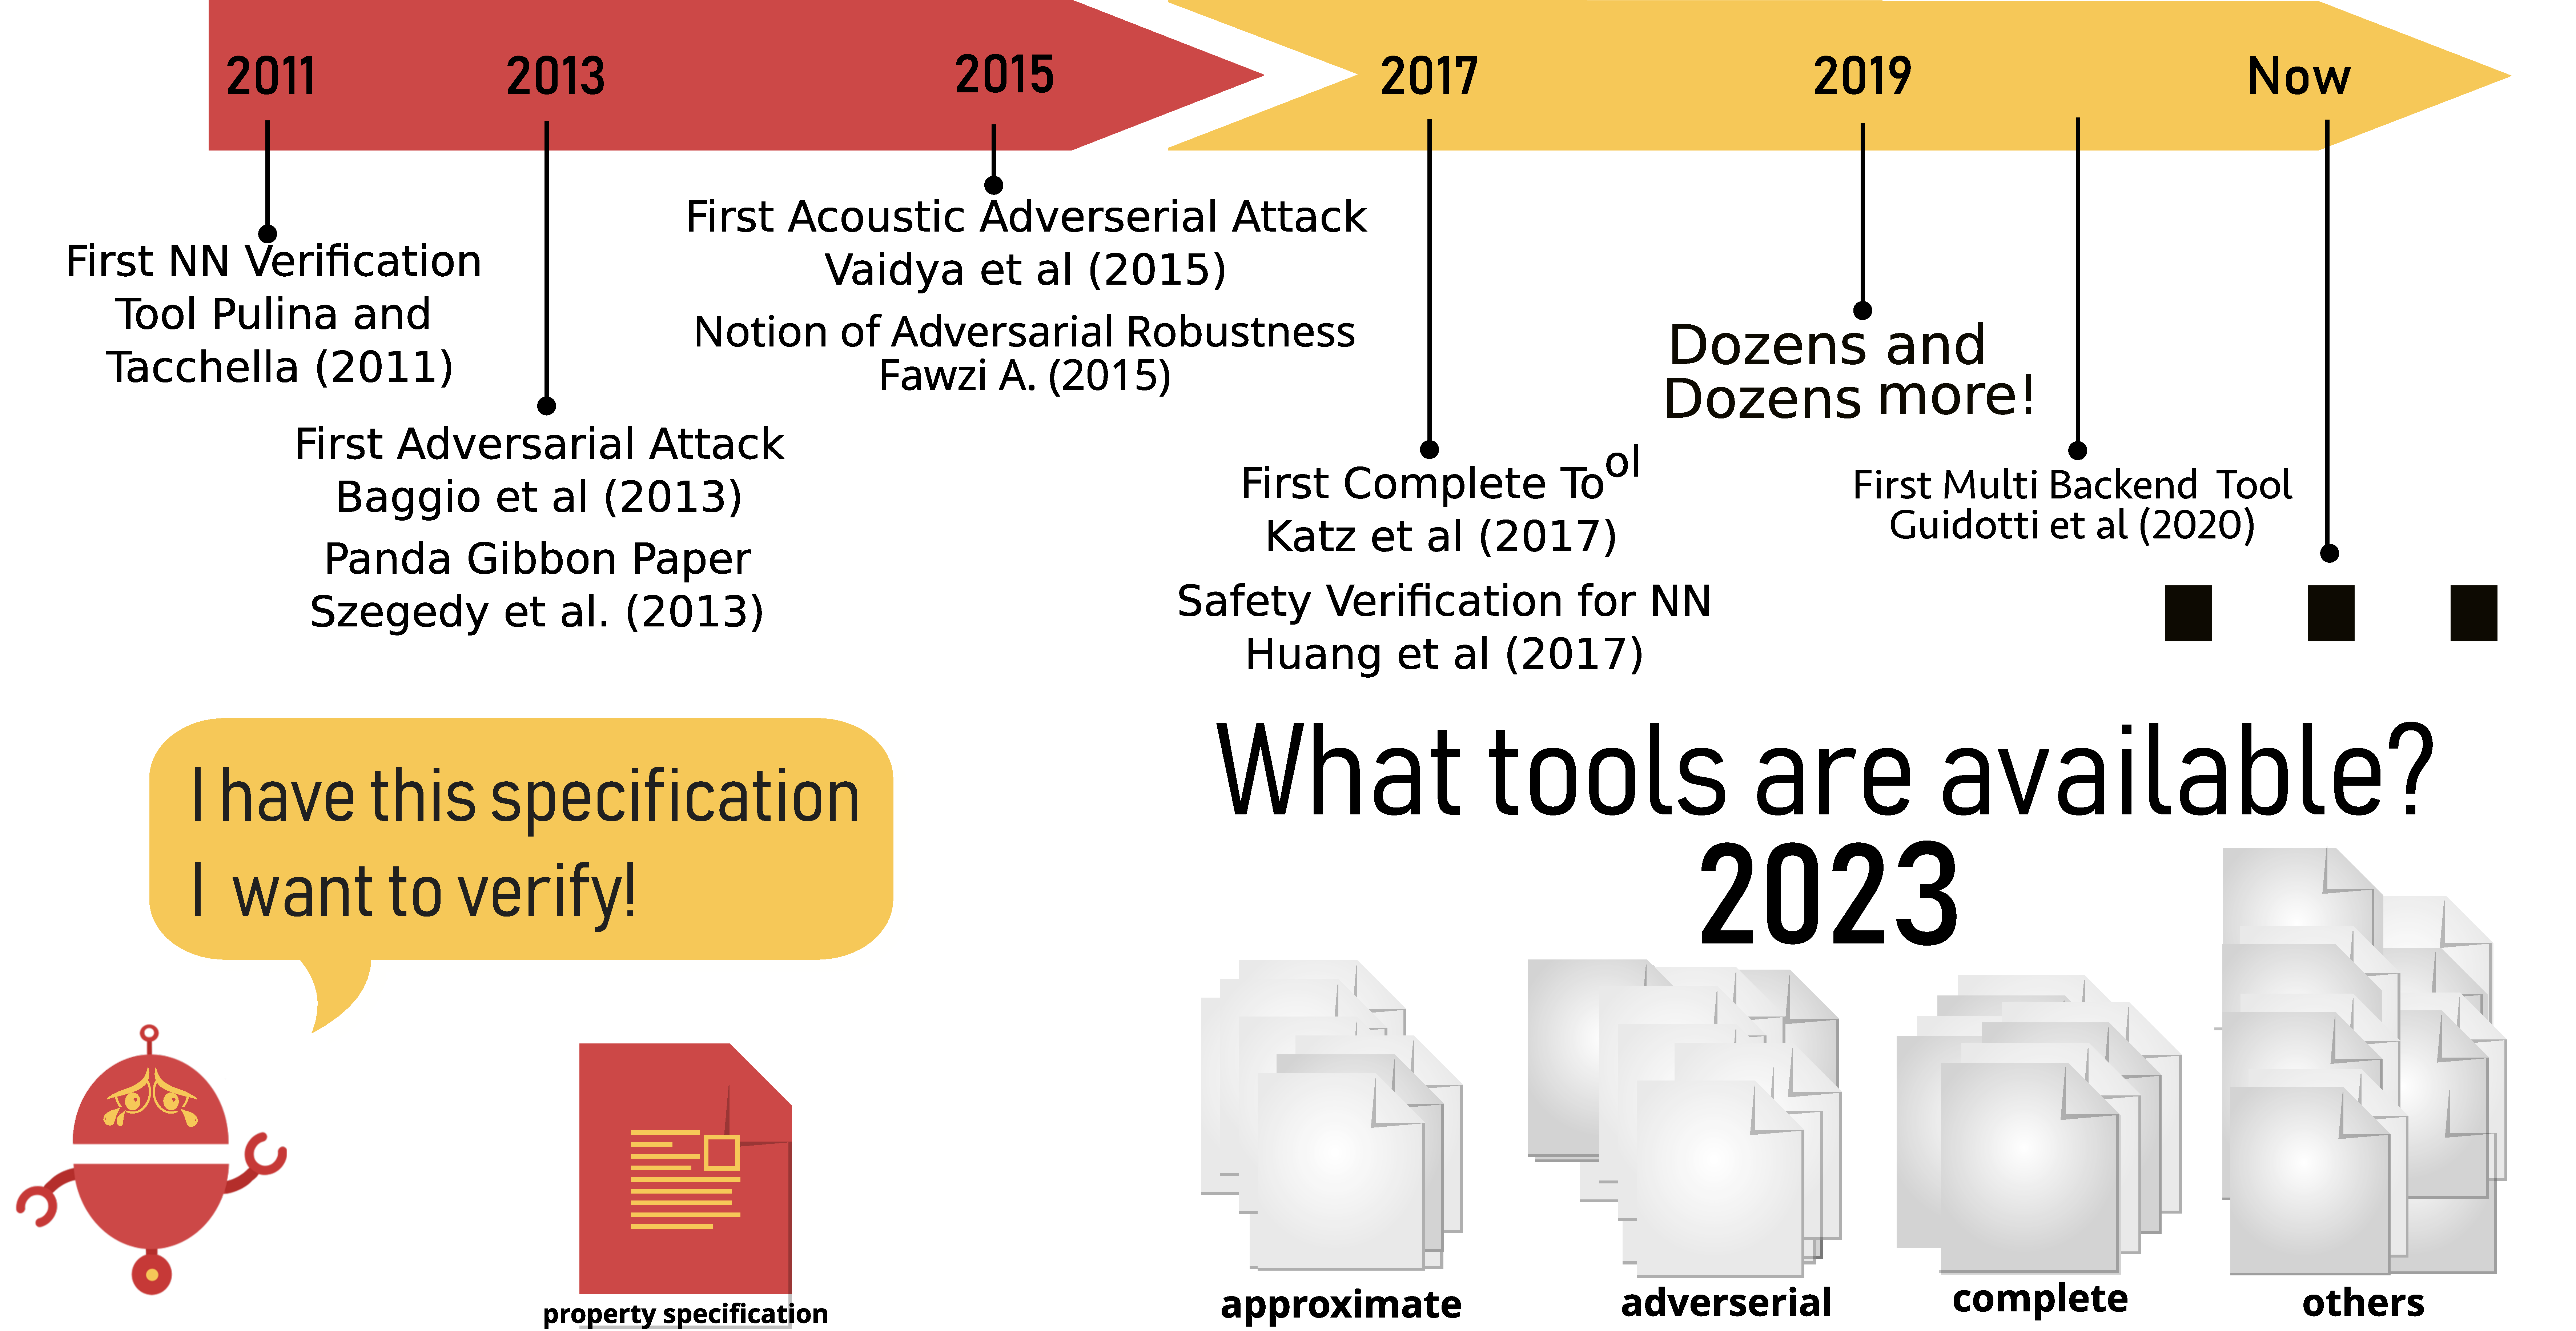
\includegraphics[width=0.9\textwidth]{img/first-slide-2022.pdf}}
\end{frame}






\begin{frame}
\frametitle{Current Verifier Landscape}

A whole range of domain-specific verifiers exist:
\begin{itemize}
\pause
\item Marabou (SMT technology)
\pause
\item ERAN (abstract interpretation + MILP)
\pause
\item Verisig (interval arithmetic)
\item AlphaBetaCROWN (linear bound propagation)
\item $\ldots $
\end{itemize}

\begin{block}{International Standards and Competitions}
https://www.vnnlib.org/
\end{block}

\pause
Marabou is our current choice as it is complete, and the set of expressible queries is large!

  \uncover<2->{
    {\footnotesize
 \begin{thebibliography}{99}
 \beamertemplatearticlebibitems
\bibitem{1}{Guy Katz, Clarke Barrett, D. Dill, K. Julian, and M. Kochenderfer. Reluplex: An Efficient SMT Solver for Verifying Deep Neural Networks. In CAV, 2017.}
 \end{thebibliography}}}

\end{frame}

\section{The lifecycle of neural network verification}


\begin{frame}
\frametitle{The lifecycle of neural network verification}

\begin{center}
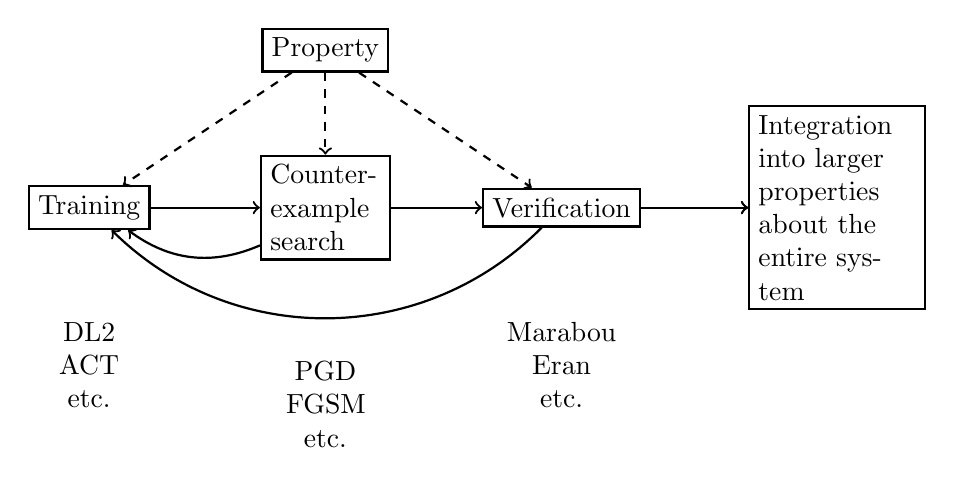
\begin{tikzpicture}[thick,
    set/.style = {circle,
        minimum size = 3cm}]

% Set A
\node[rectangle,draw] (A) at (0,4) {Property};

\onslide<2->{
\node[rectangle,draw] (B) at (-3,2) {Training};}
\onslide<2->{
\node[text width=1cm, align=center] at (-3,0) {DL2 ACT etc.};
}

\onslide<3->{\node[rectangle,draw,text width=1.4cm] (C) at (0,2) {Counter-example search};}
\onslide<3->{
\node[text width=1cm, align=center] at (0,-0.5) {PGD FGSM etc.};
}

\onslide<4->{\node[rectangle,draw] (D) at (3,2) {Verification};}
\onslide<4->{
\node[text width=1.4cm, align=center] at (3,0) {Marabou Eran etc.};
}


 \onslide<5->{\node[rectangle,draw,text width=2cm] (E) at (6.5,2) {Integration into larger properties about the entire system};
\draw [->] (D) edge (E);
}

\onslide<2->{\draw [->, dashed] (A) edge (B);}
\onslide<3->{\draw [->, dashed] (A) edge (C);}
\onslide<4->{\draw [->, dashed] (A) edge (D);}

\onslide<6->{\draw [->] (B) edge (C);}
\onslide<7->{\draw [->] (C) edge (D);}
\onslide<8->{\draw [->] (D) edge (E);}

\onslide<6->{\draw [->] (C) edge[bend left] (B);}
\onslide<7->{\draw [->] (D) edge[bend left=45] (B);}
\end{tikzpicture}
\end{center}
\end{frame}

\section{Challenges and Languages}

\begin{frame}
  \frametitle{Challenges the area faces}

  \begin{itemize}[<+->]
  \item Theory: finding appropriate verification properties
\item  Solvers: undecidability of non-linear real arithmetic  and scalability of neural network verifiers
\item ML: understanding and integrating property-driven training

\item Programming: finding the right languages to support these developments
\item Complex systems: integration of neural net verification into complex systems
  \end{itemize}
\end{frame}

\begin{frame}
\vspace{5em}
\frametitle{}
  \begin{alertblock}{Some of these problems are aggravated by insufficient
  programming language or API support}

Lets look under the hood...
  \end{alertblock}

 % \begin{block}{}
%\end{block}
    \end{frame}

\begin{frame}
\frametitle{Training framework: DL2}
\vspace{-2em}
%\only<1>{
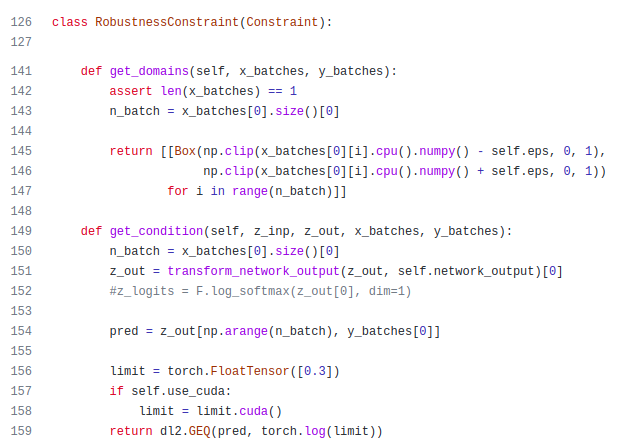
\includegraphics[width=0.6\linewidth]{img/DL2.png}
%}

%\only<2>{
%\begin{equation*}
%\forall x : \distance{x}{\hat{x}} \leq \epsilon \Rightarrow \distance{f(x)}{f(\hat{x})} \leq \delta
%\end{equation*}
%}

  \uncover<1->{
    {\scriptsize
 \begin{thebibliography}{99}
 \beamertemplatearticlebibitems
\bibitem{1}{Fischer, M., Balunovic, M., Drachsler-Cohen, D., Gehr, T., Zhang, C., and
Vechev, M. T.
DL2: training and querying neural networks with logic.
In Proc. of the 36th Int. Conf. Machine Learning, ICML 2019}
 \end{thebibliography}}}

\end{frame}

\begin{frame}
\frametitle{Training framework: ART}
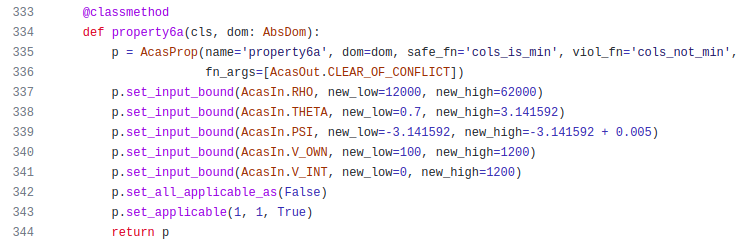
\includegraphics[width=1\linewidth]{img/art.png}

  \uncover<1->{
    {\scriptsize
 \begin{thebibliography}{99}
 \beamertemplatearticlebibitems
\bibitem{1}{Lin, X., Zhu, H., Samanta, R., and Jagannathan, S. (2020).
Art: Abstraction refinement-guided training for provably correct neural
networks.
In FMCAD 2020}
 \end{thebibliography}}}
\end{frame}

\begin{frame}
\frametitle{Verification framework: Marabou }
\vspace{-2em}

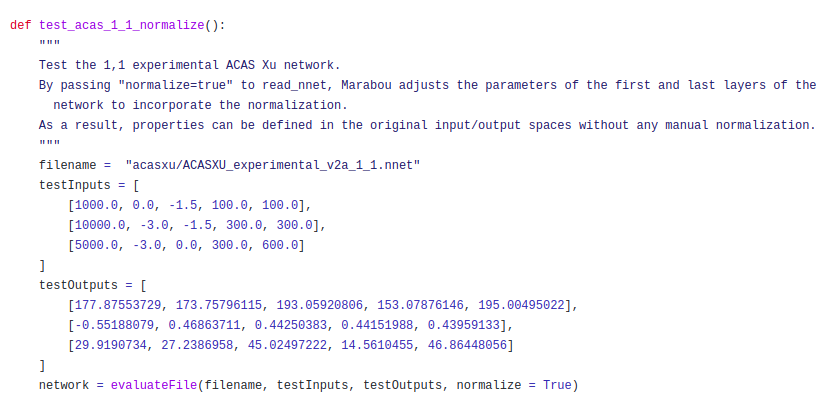
\includegraphics[width=0.8\linewidth]{img/marabou.png}

  \uncover<1->{
    {\scriptsize
 \begin{thebibliography}{99}
 \beamertemplatearticlebibitems
\bibitem{1}{Katz, G., Huang, D. A., Ibeling, D., Julian, K., Lazarus, C., Lim, R., Shah, P.,
Thakoor, S., Wu, H., Zeljic, A., Dill, D. L., Kochenderfer, M. J., and Barrett,
C. W. (2019).
The Marabou framework for verification and analysis of deep neural
networks.
In CAV 2019}
 \end{thebibliography}}}
\end{frame}

\begin{frame}
\frametitle{Verification framework: ERAN}
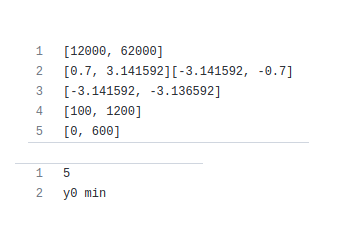
\includegraphics[width=0.5\linewidth]{img/eran.png}

 \uncover<1->{
    {\scriptsize
 \begin{thebibliography}{99}
 \beamertemplatearticlebibitems
\bibitem{1}{Singh, G., Gehr, T., Püschel, M., and Vechev, M. T. (2019).
An abstract domain for certifying neural networks.
PACMPL, 3(POPL):41:1–41:30.}
 \end{thebibliography}}}
\end{frame}

\begin{frame}
\frametitle{Verification property language: VNNLIB}
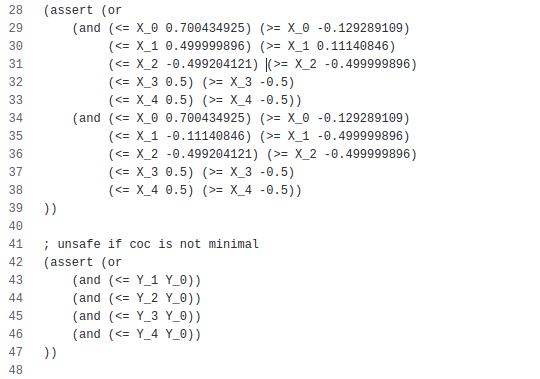
\includegraphics[width=0.7\linewidth]{img/vnnlib.png}
\end{frame}




\begin{frame}
\frametitle{Recap: What are the problems from the PL perspective?}

\pause
\begin{itemize}
\item[$I^O$] Interoperability -- properties are not portable between training/counter-example search/ verification.
\pause
\item[$I^{P}$] Interpretability -- code is not easy to understand.
\pause
\item[$I^{\int}$] Integration -- properties of networks cannot be linked to larger control system properties.
\pause
\item[$E^G$] Embedding gap -- little support for translation between problem space (as in original spec) and input space (at neural network level).
\end{itemize}

\alert{Vehicle is designed to address all of these problems}

\end{frame}

\begin{frame}
\frametitle{Vehicle ...}
\centering
\vspace{-2em}
 \textbf{ is a domain-specific functional language for writing} \\ \textbf{ high-level property specifications for neural networks}

\begin{center}
\begin{tikzpicture}[thick,
    set/.style = {circle,
        minimum size = 3cm}]

% Set A
\node[rectangle,draw] (A) at (1.5,5) {\alert<1->{Property in Vehicle}};

\node[rectangle,draw] (B) at (-3,2) {\alert<4->{Training}};
\node[text width=2cm, align=center] at (-3,0.7) {\alert<4->{DL2 or other DL (native)}};

\node[rectangle,draw, dashed,text width=1.4cm] (C) at (0,2) {\alert<5->{Counter-example search}};
\node[text width=2cm, align=center] at (0,0.7) {\alert<5->{PGD FGSM etc.}};

\node[rectangle,draw] (D) at (3,2) {\alert<3->{Verification}};
\node[text width=2cm, align=center] at (3,0.7) {\alert<3->{Marabou} Eran etc.};

\node[rectangle,draw] (E) at (6,2) {\alert<6->{Integration}};
\node[text width=2cm, align=center] at (6,0.7) {\alert<6->{Agda} Imandra KeymaeraX etc.};

\draw [->] (A) edge (B);
\draw [->, dashed] (A) edge (C);
\draw [->] (A) edge (D);
\draw [->] (A) edge (E);
%\draw [->, dashed] (A) edge (C);
\draw [->] (B) edge (C);
\draw [->] (C) edge (D);
\draw [->] (D) edge (E);

\onslide<1->{
\node[rectangle,draw,fill=normal text.bg] (D) at (1.5,4) {\alert<2->{Analysis \& informative error messages}};
}


\end{tikzpicture}
\end{center}
\end{frame}

\begin{frame}
\frametitle{Other Similar APIs}
  \vspace{-2em}
\footnotesize{
\begin{itemize}%[<+->]

\item Socrates [in Python]:  Given a spec and a network (in JSON), calls different NN verifiers.
  {\scriptsize
 \begin{thebibliography}{99}
 \beamertemplatearticlebibitems
\bibitem{1}{L. H. Pham, J. Li, and J. Sun. 2020. SOCRATES: Towards a Unified Platform for Neural Network Verification.
CoRR abs/2007.11206.}
 \end{thebibliography}}

 {\alert {\small Left unresolved: $I^O$, $I^P$, $I^{\int}$, $E^G$}}

 \pause
 \item NeVer 2.0 [in Python]: added training, prunning and quantization to this functionality.
  {\scriptsize
 \begin{thebibliography}{99}
 \beamertemplatearticlebibitems
\bibitem{1}{D. Guidotti, L. Pulina, and A. Tacchella. 2020. NeVer 2.0: Learning, Verification and Repair of Deep Neural
Networks. CoRR abs/2011.09933.}
 \end{thebibliography}}

  {\alert {\small Resolved: $I^O$ (partially). Left untesolved: $I^P$, $I^{\int}$, $E^G$ }}

 \pause

 \item CoCoNet [in Python]: NN format converter with GUI
  {\scriptsize
 \begin{thebibliography}{99}
 \beamertemplatearticlebibitems
\bibitem{1}{D. Guidotti, A. Tacchella, L. Pulina, S. Demarchi 2023. \url{http://neuralverification.org/}}
 \end{thebibliography}}

  {\alert {\small Resolved: $I^P$ (partially). Left untesolved: $I^O$, $I^{\int}$, $E^G$ }}

 \pause

 \item Caisar [in OCAML] -- general specification language and connection to several NN Verifiers

{\scriptsize
 \begin{thebibliography}{99}
 \beamertemplatearticlebibitems
\bibitem{1}{J. Girard-Satabin, M. Alberti, F. Bobot, Z. Chihani, and A. Lemesle. 2022. CAISAR: A platform
for Characterizing Artificial Intelligence Safety and Robustness. In AISafety.}
 \end{thebibliography}}

 {\alert {\small Resolved: $I^P$, $I^{\int}$. Left unresolved: $I^O$,  $E^G$ }}

\end{itemize}}

\end{frame}

\section{\textbf{Vehicle}'s Role and Purpose of this Tutorial}

\begin{frame}
\frametitle{\textbf{Vehicle}'s Aim...}

\alert{... is to resolve the problems $I^O$, $I^P$, $I^{\int}$, $E^G$}
\pause

... and support community's effort towards resolution of the ``Grand Challenges"

\end{frame}

  \begin{frame}
  \frametitle{``Grand Challenges"  \& \textbf{Vehicle}}
  \footnotesize{
  \begin{itemize}
  \item Theory: finding appropriate verification properties
\item  Solvers: undecidability of non-linear real arithmetic  and scalability of neural network verifiers
\item \alert{ML: understanding and integrating property-driven training}
\item \alert{Programming: finding the right languages to support these developments}
\item \alert{Complex systems: integration of neural net verification into complex systems}
  \end{itemize}}

\end{frame}

\begin{frame}
\frametitle{\textbf{Vehicle} among other disciplines}
  \begin{center}
  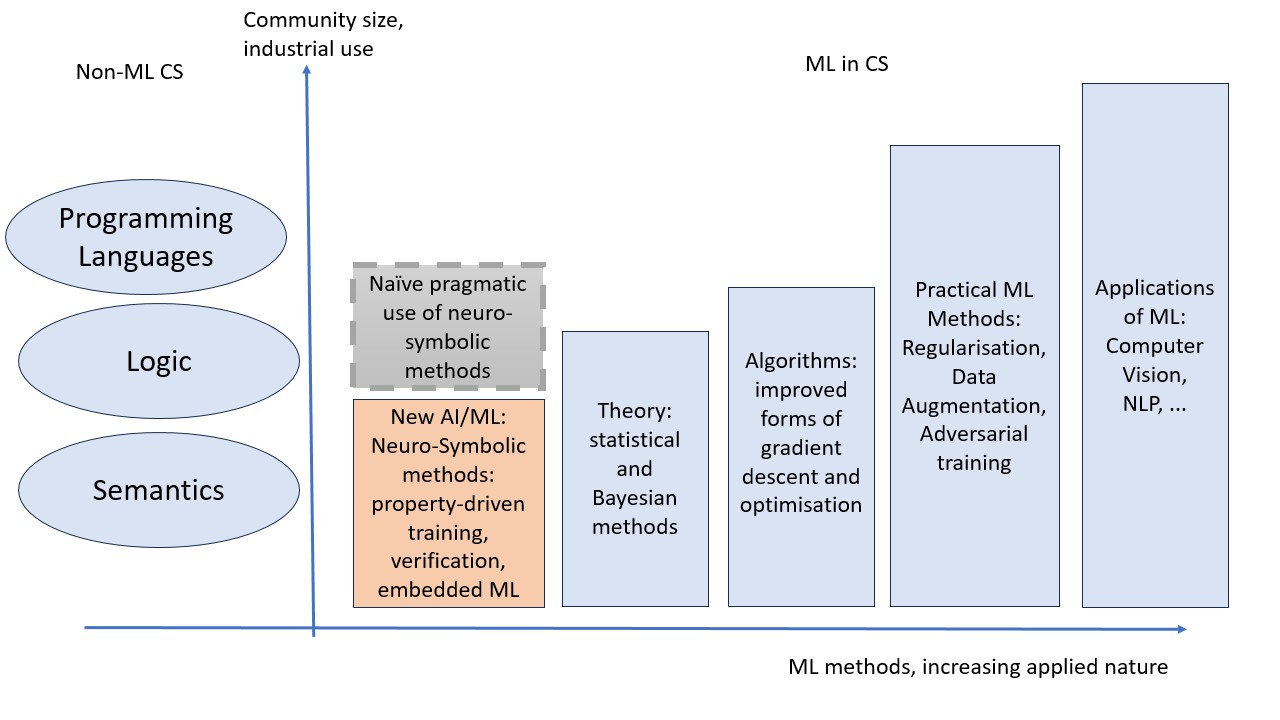
\includegraphics[scale=.32]{img/Slide1.jpg}
  \end{center}
\end{frame}


 \begin{frame}
  \frametitle{\textbf{Vehicle} Architecture}
     \begin{center}
      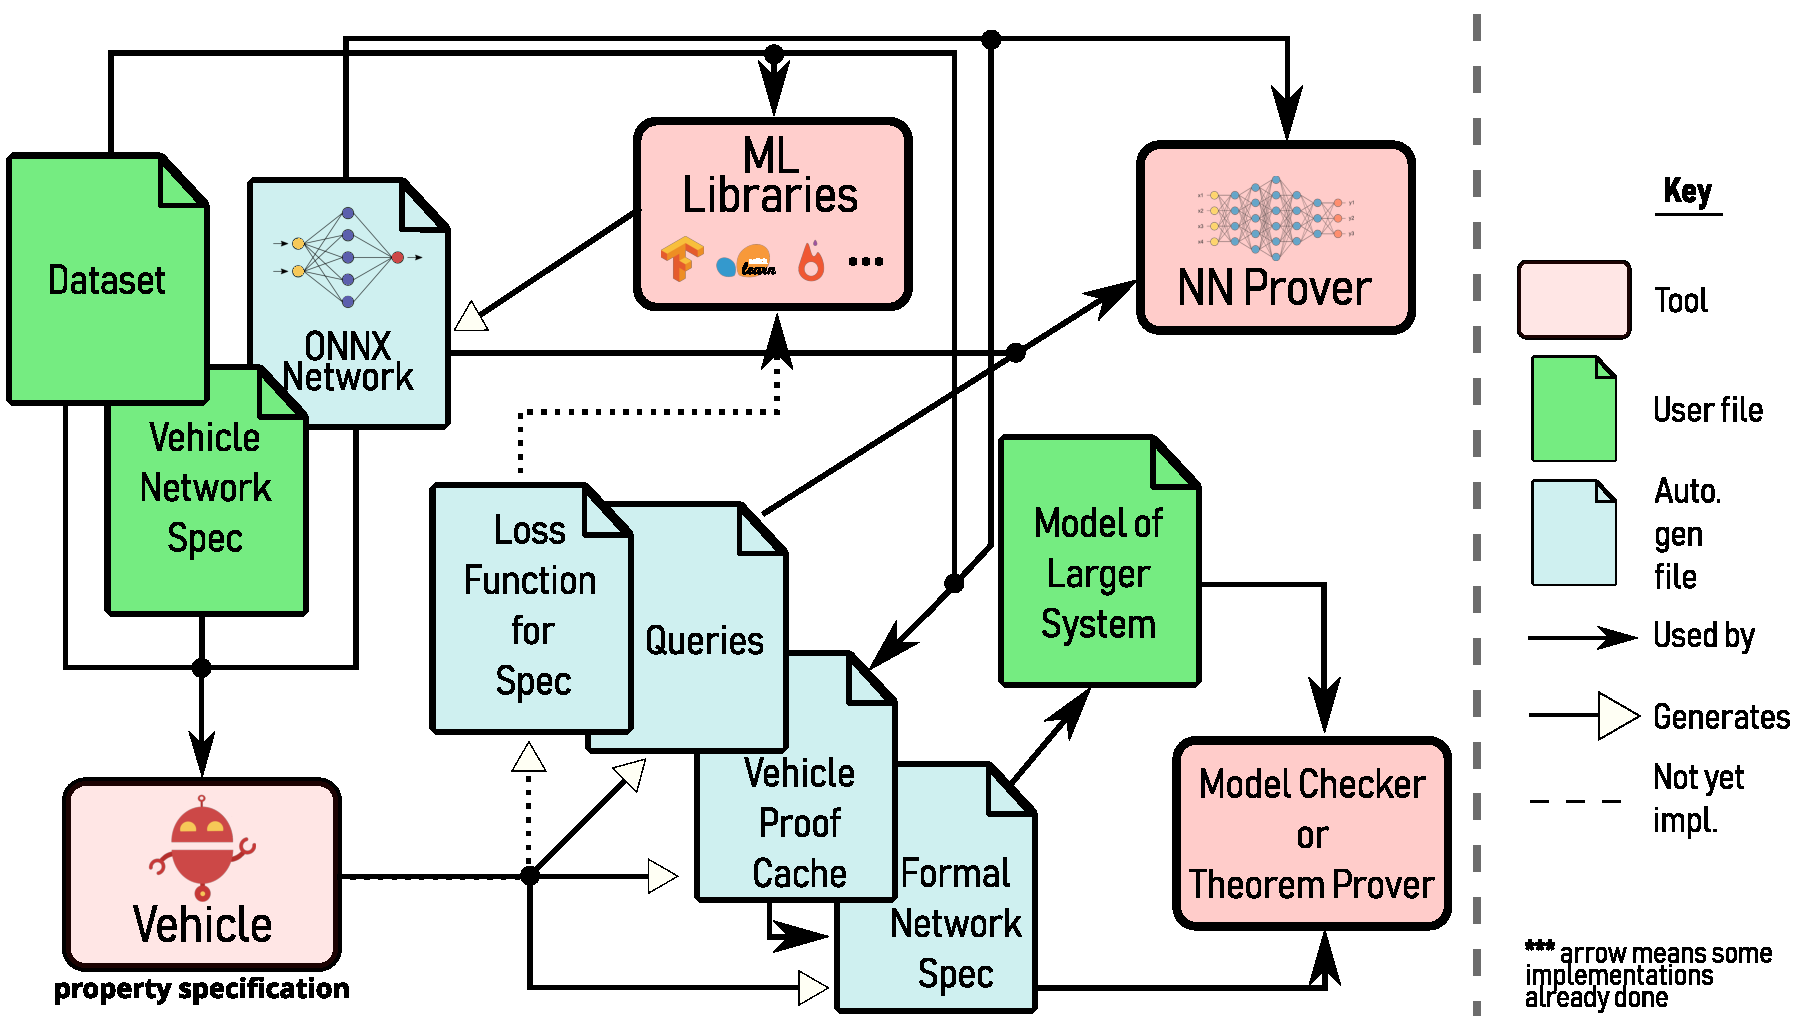
\includegraphics[width=0.7\textwidth]{img//vehicle-overview.pdf}
    \end{center}

  \end{frame}

\begin{frame}
\frametitle{Sources}

    {\scriptsize
 \begin{thebibliography}{99}
 \beamertemplatearticlebibitems
\bibitem{1}{M. Daggitt, R. Atkey, W. Kokke, E. Komendantskaya, L. Arnaboldi:
Compiling Higher-Order Specifications to SMT Solvers: How to Deal with Rejection Constructively. CPP 2023}

\bibitem{2}{N. Slusarz, E. Komendantskaya, M. Daggitt, R. Stewart, K. Stark:
Logic of Differentiable Logics: Towards a Uniform Semantics of DL. LPAR 2023.}

\bibitem{3}{
 	Matthew L. Daggitt, Wen Kokke, Robert Atkey, Luca Arnaboldi, Ekaterina Komendantskaya:
Vehicle: Interfacing Neural Network Verifiers with Interactive Theorem Provers. FOMLAS 2022}

\bibitem{4}{Vehicle Team: The Vehicle language: \url{https://github.com/vehicle-lang} 2023.}

\bibitem{5}{M.Daggitt and W.Kokke: Vehicle User Manual. \url{https://vehicle-lang.readthedocs.io} 2023.}

\bibitem{6}{The Vehicle team: Vehicle Tutorial \url{https://vehicle-lang.github.io}. 2023. Tutorial code repository \url{https://github.com/vehicle-lang/vehicle-tutorial}. }
 \end{thebibliography}}

\end{frame}

\begin{frame}
\frametitle{Purpose of this Tutorial...}

\begin{block}{}
\begin{itemize}

\item Discuss challenges in NN verification ("grand" and technical)

\item Understand how logic and PL semantics can contribute in this domain

\item Introduce \textbf{Vehicle} specification language at the user level

\item Give you a  bit of practice with NN verification and gather feedback
\end{itemize}
\end{block}

\end{frame}

\begin{frame}
\frametitle{Plan for the rest of this tutorial}

\begin{itemize}
\item Before coffee break:
\begin{itemize}
\item Brief introduction to \textbf{Vehicle} specification language
\item Neural Network Robustness: an iconic verification case


\end{itemize}

\item During and after the break:

\begin{itemize}

\item \alert{Exercise session:} write and verify a \textbf{Vehicle} spec

\footnotesize{Tutorial pages: \url{https://vehicle-lang.github.io}}

%\begin{itemize}
%\item for writing a spec, install vehicle: just run
%\texttt{pip install vehicle}
%\item for verifying a spec, you also need Marabou installed
%\texttt{pip install marabou}
%\end{itemize}

 Join tutorial Slack channel via the tutorial page, to ask questions

\end{itemize}

\item After the break:
\begin{itemize}



\item Property-driven training in Vehicle
%\item Demo of large system integration in Vehicle
\item Large system integration

\item Application areas for NN Verification
\end{itemize}


\end{itemize}

\end{frame}

\end{document}
